\chapter{Simulation and Stability}
\label{chap:simulation}

This chapter studies the behaviour of the arbitrage-free encoder--decoder model when it is used beyond curve reconstruction. In particular, we ask whether the learned latent dynamics can be used to generate yield curve scenarios, comprising zero-coupon bond price curves and swap-rate curves, by simulating latent paths under the model's risk-neutral dynamics.

To investigate this, we consider two models. The first is the arbitrage-free encoder--decoder model introduced in Chapter \ref{chap:encoderdecodermodel}, referred to here as the \textit{baseline}. The second is a \textit{stable} model proposed in this Chapter, which restricts the model components of the baseline in order to produce more controlled simulated paths. These modifications are described in Section~\ref{sec:stability_analysis}, after which the two models are compared empirically to assess whether the stable model achieves more controlled simulated scenarios without sacrificing reconstruction accuracy.


%========================================================
\section{Simulation Setup}
\label{sec:simulation-latent-dynamics}
%========================================================

This section describes the simulation procedure common to both models. Starting from an observed swap-rate curve on an arbitrary initial date, the encoder maps the curve to an initial latent state, which is then simulated forward under the model's learned risk-neutral dynamics. At each time step, the latent state is sent through the decoder to produce a zero-coupon bond price curve and the corresponding swap-rate curve.

Let \(\mathbf{S}_0 \in \mathbb{R}^8\) denote the observed market swap curve on a chosen initial date. The trained encoder \eqref{eq:linear_encoder} maps this curve to an initial latent state,
\[
z_0 = A_1\mathbf{S}_0 \in \mathbb{R}^{\ell},
\]
where \(\ell\) denotes the latent dimension. Starting from \(z_0\), the latent state is simulated forward under the learned risk-neutral dynamics \eqref{latentdynamics},
\[
dz_t = \mu(z_t)\,dt + \sigma(z_t)\,dW_t^{\mathbb{Q}},
\]
where \(W_t^{\mathbb{Q}}\) is an \(\ell\)-dimensional Brownian motion under the risk-neutral measure \(\mathbb{Q}\), \(\mu(z_t)\) is the learned drift vector and \(\sigma(z_t)\) is the volatility matrix defined in Section~\ref{subsec:neural-modelling-dynamics}.

%Under the regularity conditions established in Appendix~\ref{app:???}, the latent SDE admits a unique non-explosive solution for both models considered in this chapter, ensuring that the simulated processes are mathematically well defined.

The latent SDE is discretised using the Euler--Maruyama scheme \citep{Glasserman2004}. For a time step \(\Delta t>0\) and grid points \(t_n=n\Delta t\), \(n=0,1,\ldots,N\), where $N$ is the total number of steps and \(T=N\Delta t\) is the horizon, the simulated paths satisfy
\[
z_{t_{n+1}}
=
z_{t_n}
+
\mu(z_{t_n})\,\Delta t
+
\sigma(z_{t_n})\,\Delta W_n,
\qquad
\Delta W_n \sim \mathcal{N}(0,\Delta t\,I_{\ell}).
\]
From the simulated latent path, the short-rate path is obtained using the short-rate specification \eqref{shortratedynamic},
\[
r_{t_n}=\tilde r(z_{t_n}),
\qquad n=0,1,\ldots,N,
\]
The pathwise discount factor is given by
\[
D_{t_n}
=
\exp\left(
-
\int_{0}^{t_n}
\tilde{r}(z_{s})\,ds 
\right)
\]
It is approximated using the trapezoidal rule \citep{Glasserman2004}, with \(\tilde{r}_{t_k}:=\tilde{r}(z_{t_k})\):
\[
D_{t_n}
\approx
\exp\!\left(
-
\sum_{k=0}^{n-1}
\frac{\tilde{r}_{t_k}+\tilde{r}_{t_{k+1}}}{2}\,\Delta t
\right).
\]
For each simulated latent state \(z_{t_n}\), the zero-coupon bond curve is recovered through the decoder by solving the no-arbitrage ODE system \eqref{ODEB}--\eqref{ODEA} numerically,
\[
P(z_{t_n},\tau)
=
\exp\bigl(
A_{z_{t_n}}(\tau)
-
B_{z_{t_n}}(\tau)\mathcal{G}(z_{t_n},\tau)
\bigr).
\]
Hence, each simulated path yields a time series of latent states, short rates, discount factors, and zero-coupon bond curves, from which the corresponding swap-rate curves are obtained using \eqref{estimatedswaprates}.

%========================================================
\section{The Stable Model}
\label{sec:stability_analysis}
%========================================================

The baseline latent dynamics admit a unique non-explosive solution under the regularity conditions verified in Section~\ref{sec:baseline_existence_uniqueness}, establishing that the model is mathematically well-defined independently of any simulation scheme. When simulated over a multi-year horizon, however, this does not alone ensure that simulated paths remain on a controlled scale. Several stability issues may arise, stemming from the drift, diffusion, and short rate components of the latent model. The following identifies these issues and the corresponding modifications introduced in the stable model.

\begin{description}[
    style=unboxed,
    leftmargin=0pt,
    labelindent=0pt,
    labelsep=0.5em
]
\item[Drift stability.] The baseline drift is affine,
\[
\mathcal{K}(z)=Mz+N,
\qquad
M\in\mathbb{R}^{\ell\times\ell},
\quad
N\in\mathbb{R}^{\ell},
\]
where \(M\) and \(N\) are learned parameters. Mean reversion is a property to be imposed on the drift to ensure that the latent state fluctuates around a long-run equilibrium rather than drifting without bound. The baseline model does not guarantee this, since \(M\) is unconstrained.

Whether the drift is mean-reverting is determined by the eigenvalues 
of $M$, as the following result establishes. Note that, in what follows, a dot denotes differentiation with respect to time.

\begin{proposition}[Mean reversion condition]
Let $M\in\mathbb{R}^{\ell\times\ell}$ be invertible and diagonalisable
with eigenvalues $\lambda_1,\ldots,\lambda_\ell\in\mathbb{C}$, and let
$N\in\mathbb{R}^{\ell}$. The deterministic system $\dot{z}_t = Mz_t + N$
has a unique fixed point $z^* = -M^{-1}N$ and is globally asymptotically
stable about $z^*$ if and only if $\operatorname{Re}(\lambda_i) < 0$
for all $i$.
\label{prop:meanreversion}
\end{proposition}

\begin{proof}
Since $M$ is invertible, the fixed point equation $Mz^* + N = 0$ has
the unique solution $z^* = -M^{-1}N \in \mathbb{R}^{\ell}$. Define
$y_t := z_t - z^*$. Since $z^*$ is constant, $\dot{y}_t = \dot{z}_t$,
and using $Mz^* + N = 0$,
\[
    \dot{y}_t = Mz_t + N = M(y_t + z^*) + N
    = My_t + \underbrace{Mz^* + N}_{=\,0} = My_t,
\]
so the deviation satisfies $\dot{y}_t = My_t$ with initial condition
$y_0 = z_0 - z^*$. The unique solution is $y_t = e^{Mt}y_0$, where
$e^{Mt} := \sum_{k=0}^{\infty}(Mt)^k/k!$. To verify, differentiate
the series term by term,
\[
    \frac{d}{dt}e^{Mt}
    = \sum_{k=1}^{\infty}\frac{M^k k t^{k-1}}{k!}
    = M\sum_{k=1}^{\infty}\frac{M^{k-1}t^{k-1}}{(k-1)!}
    = M\sum_{j=0}^{\infty}\frac{(Mt)^j}{j!}
    = Me^{Mt},
\]
so $\dot{y}_t = Me^{Mt}y_0 = My_t$, confirming the solution. Since $M$
is diagonalisable, let $v_1,\ldots,v_\ell$ be a basis of eigenvectors
satisfying $Mv_i = \lambda_i v_i$, and write $y_0 = \sum_{i=1}^{\ell}
c_i v_i$ for unique coefficients $c_i \in \mathbb{C}$. Using
$M^k v_i = \lambda_i^k v_i$ by induction, $e^{Mt}v_i = e^{\lambda_i t}v_i$,
and by linearity,
\[
    y_t = \sum_{i=1}^{\ell} c_i e^{\lambda_i t} v_i.
\]
Writing $\lambda_i = \alpha_i + \mathrm{i}\beta_i$, we have
$|e^{\lambda_i t}| = e^{\alpha_i t}$ since $|e^{\mathrm{i}\beta_i t}|
= \sqrt{\cos^2(\beta_i t) + \sin^2(\beta_i t)} = 1$, and the triangle
inequality gives
\[
    \|y_t\| \leq \sum_{i=1}^{\ell} |c_i|\,e^{\alpha_i t}\|v_i\|.
\]
If $\alpha_i=\operatorname{Re}(\lambda_i) < 0$ for all $i$, every term decays
exponentially to zero, so $\|y_t\| \to 0$ and hence $z_t \to z^*$ for
every initial condition $z_0$. Conversely, if
$\alpha_j=\operatorname{Re}(\lambda_j) \geq 0$ for some $j$, choose $y_0 = v_j$
so that $y_t = e^{\lambda_j t}v_j$ and
$\|y_t\| = e^{\alpha_j t}\|v_j\|$. If $\alpha_j > 0$ this grows
unboundedly; if $\alpha_j = 0$ it remains equal to $\|v_j\| > 0$ for
all $t \geq 0$. In either case $z_t \not\to z^*$, so asymptotic
stability fails. The full result without the diagonalisability
assumption is given by \citet[Theorem~4.5]{Khalil2002}.
\end{proof}


To enforce mean reversion, the stable variant replaces the unconstrained drift
matrix with the parametrisation
\[
M = -\underbrace{\left(V^\top V+\varepsilon I_\ell\right)}_{=:\,A},
\qquad
V\in\mathbb{R}^{\ell\times\ell},
\quad
\varepsilon>0.
\]
Since $(V^\top V)^\top = V^\top(V^\top)^\top = V^\top V$, the matrix
$A = V^\top V + \varepsilon I_\ell$ is real symmetric, and the spectral theorem \citep[Theorem~6.4.2]{HesselholtWahl2016}
therefore guarantees that $A$, and hence $M = -A$, is
orthogonally diagonalisable. For any unit eigenvector $v$ satisfying
$Av = \lambda_i(A) v$,
\[
\lambda_i(A) = v^\top A v = \|Vv\|^2 + \varepsilon\|v\|^2 \geq \varepsilon,
\]
so $A$ is strictly positive definite with all eigenvalues bounded below
by $\varepsilon > 0$. It follows that $M$ is invertible and
\[
\lambda_i(M) = -\lambda_i(A) \leq -\varepsilon < 0.
\]
The assumptions of Proposition~\ref{prop:meanreversion} are therefore satisfied, and global asymptotic stability about $z^*$ holds by construction.

%\begin{remark}
%    The scalar analogue of the stable parametrisation is the Ornstein--Uhlenbeck process, where $M=-\kappa$ for some $\kappa>0$, so that $\dot{z}_t=-\kappa(z_t-\mu)$ is mean-reverting with speed $\kappa$. The stable variant generalises this to the multivariate setting by replacing the scalar $-\kappa$ with the matrix $M=-(V^\top V+\varepsilon I_\ell),$ which plays the role of the mean reversion speed matrix.
%\end{remark}


\item[Diffusion scale.] The baseline volatility network \(\mathcal{H}\) recovers individual volatility levels as
\[
\sigma_i(z)=\exp([\mathcal{H}(z)]_i).
\]
which ensures strict positivity, but places no upper bound on \(\sigma_i(z)\). Large volatility values amplify the Brownian shock term, and even a mean-reverting drift may fail to keep simulated paths on a controlled scale if the diffusion term is sufficiently large.



The stable model therefore bounds the volatility levels \textit{explicitly}. Instead of using an unrestricted exponential transformation, it sets
\[
\log\sigma_i(z)
=
\log\sigma_{\min}
+
\bigl(\log\sigma_{\max}-\log\sigma_{\min}\bigr)
\operatorname{sigmoid}\bigl(u_i(z)+b_i\bigr),
\]
where \(u_i(z)\) is the \(i\)-th raw network output before the volatility transformation, \(b_i\) is a learnable bias term, and
\[
0<\sigma_{\min}<\sigma_{\max}
\]
are fixed numerical bounds. Since the sigmoid function takes values in \((0,1)\), we have
\[
\log\sigma_i(z)
\in
\bigl(\log\sigma_{\min},\log\sigma_{\max}\bigr),
\]
and therefore
\[
\sigma_i(z)\in(\sigma_{\min},\sigma_{\max})
\qquad
\forall z\in\mathbb{R}^{\ell}.
\]

The bounds $\sigma_{\min}$ and $\sigma_{\max}$ are fixed numerical hyperparameters, not learned from data.


\item[Correlation structure.] The volatility levels alone do not determine the full diffusion matrix. In the baseline model, the last $\ell(\ell-1)/2$ outputs of $\mathcal{H}(z)$ are used as raw parameters for the pairwise correlations, and are denoted
\[
v_{ij}(z) := [\mathcal{H}(z)]_{\ell+k}, \qquad k = 1,\ldots,\ell(\ell-1)/2,
\]
where $k$ enumerates the pairs $(i,j)$ with $i=2,\ldots,\ell$ and $j=1,\ldots,i-1$ in row-wise order. Each raw parameter is mapped to a pairwise correlation via
\[
\rho_{ij}(z) = \tanh \bigl(v_{ij}(z)\bigr) \in (-1,1).
\]
While each $\rho_{ij}$ lies in $(-1,1)$, specifying pairwise correlations  independently does not guarantee that the full correlation matrix is  positive definite for $\ell \geq 3$.

The stable model therefore constructs the correlation matrix through a 
hyperspherical Cholesky representation \citep{PourahmadiWang2015}. The outputs $v_{ij}(z)$ are instead transformed into angles via
\[
\theta_{ij}(z) = \pi\,\operatorname{sigmoid} \bigl(v_{ij}(z)\bigr) \in (0,\pi),
\]
which are used to construct $C_\theta(z)$ such that $R(z) = C_\theta(z)C_\theta(z)^\top$ is symmetric, positive definite with unit diagonal, and hence a valid correlation matrix by construction for any $\ell$.

\item[Short-rate behaviour.] In the baseline model, the short-rate network uses the centered soft-step activation from \eqref{eq:activation}:
\[
\tilde r(z)
=
W_2\psi(W_1z),
\qquad
\psi(x)=\frac{1}{1+e^{-x}}-\frac12.
\]
Since each component of \(\psi(W_1z)\) lies in \((-1/2,1/2)\), the short rate is bounded for all latent states by:
\[
|\tilde r(z)|
=
|W_2\psi(W_1z)|
\leq
\sum_j |(W_2)_j|\,|\psi((W_1z)_j)|
\leq
\frac12\|W_2\|_1.
\]
However, the bound is set by the learned weights. When the simulated latent state becomes large, \(W_1z\) grows in magnitude and the activation is pushed toward its limiting values \(\pm 1/2\), pinning the short rate near a network-implied ceiling or floor. The short rate stays finite, but only because the activation saturates.

The stable model instead parametrises the short rate as
\[
r(z)
=
r_{\mathrm{center}}
+
r_{\mathrm{scale}}\tanh(\mathcal{R}(z)),
\]
where \(\mathcal{R}(z)\) is the neural network from the baseline model described in Section~\ref{subsec:neural-modelling-dynamics} and \(r_{\mathrm{center}}\in\mathbb{R}\) and \(r_{\mathrm{scale}}>0\) are learnable parameters. To ensure positivity of the scale,
\[
r_{\mathrm{scale}}
=
\operatorname{softplus}(\eta)+s_{\min},
\]
where \(\eta\in\mathbb{R}\) is an unconstrained trainable parameter and \(s_{\min}>0\) is a small lower bound on the scale. Since \(\tanh(\mathcal{R}(z))\in(-1,1)\), the short rate satisfies
\[
r(z)
\in
\bigl(
r_{\mathrm{center}}-r_{\mathrm{scale}},
\;
r_{\mathrm{center}}+r_{\mathrm{scale}}
\bigr).
\]
The range is now set by trainable parameters rather than by activation saturation. 
\end{description}


Together, these above modifications to the components of the baseline model, define the stable model. Section~\ref{sec:verify_stable_dynamics} verifies whether there exists a unique solution to the latent dynamics under the imposed constraints for the stable model. Section~\ref{sec:sim_evidence} then compares it against the baseline through a simulation experiment, and Section~\ref{sec:sim_reconstruction_accuracy} examines whether the restrictions affect reconstruction accuracy.

%========================================================
\section{Existence and Uniqueness of the Stable Latent Dynamics}
\label{sec:verify_stable_dynamics}
%========================================================
This section verifies that the latent dynamics satisfy the sufficient conditions for existence and uniqueness stated in Proposition~\ref{prop:sde_existence}, using $L$ in place of $\sigma$ for the diffusion coefficient.

% Having introduced the restrictions defining the stable model, we now verify that its latent dynamics satisfy the sufficient conditions for existence and uniqueness stated in Proposition~\ref{prop:sde_existence}. Throughout this section, \(L_{\mathrm{st}}\) denotes the diffusion coefficient of the stable SDE, rather than \(\sigma_{\mathrm{st}}\), in order to emphasise its factor representation as the product of a diagonal volatility matrix and a correlation factor.

The stable latent dynamics are given by
\begin{equation}
    dz_t
    =
    \mu_{\mathrm{st}}(z_t)\,dt
    +
    L_{\mathrm{st}}(z_t)\,dW_t^{\mathbb Q},
    \label{eq:app_stable_sde}
\end{equation}
where
\[
    \mu_{\mathrm{st}}(z)
    =
    Mz+N,
    \qquad
    M=-(V^\top V+\varepsilon I_\ell),
    \qquad
    \varepsilon>0.
\]
The volatilities are defined by
\[
    \log \sigma_i(z)
    =
    \log \sigma_{\min}
    +
    \bigl(
        \log \sigma_{\max}
        -
        \log \sigma_{\min}
    \bigr)
    \operatorname{sigmoid}\bigl(u_i(z)\bigr),
\]
where
\[
    0<\sigma_{\min}<\sigma_{\max}<\infty.
\]
The correlation factor is constructed through the hyperspherical parameterisation described in  Appendix~\ref{app:hyperspherical_cholesky}. In particular,
\[
    \theta_{ij}(z)
    =
    \pi\,\operatorname{sigmoid}\bigl(v_{ij}(z)\bigr),
    \qquad
    1\leq j<i\leq\ell,
\]
determines the lower-triangular factor \(C_\theta(z)\). The stable volatility matrix is then
\[
    L_{\mathrm{st}}(z)
    =
    D(z)C_\theta(z),
    \qquad
    D(z)
    =
    \operatorname{diag}
    \bigl(\sigma_1(z),\ldots,\sigma_\ell(z)\bigr).
\]


\begin{description}[
    style=unboxed,
    leftmargin=0pt,
    labelindent=0pt,
    labelsep=0.5em
]

\item[Drift.]
The drift satisfies
\[
\|\mu_{\mathrm{st}}(z)-\mu_{\mathrm{st}}(y)\|
=
\|M(z-y)\|
\leq
\|M\|\,\|z-y\|,
\]
so the drift is globally Lipschitz with constant $\|M\|$.

\item[Diffusion.]

As shown in Section \ref{sec:baseline_existence_uniqueness}, the functions $u_i(z)$ and $v_{ij}(z)$ are bounded and globally Lipschitz. Since $\operatorname{sigmoid}$ is globally Lipschitz with constant $\tfrac{1}{4}$, each map
$z\mapsto\log\sigma_i(z)$ is globally Lipschitz as a composition. Moreover,
since $\operatorname{sigmoid}(\cdot)\in(0,1)$, the log-volatilities are confined
to $(\log\sigma_{\min},\log\sigma_{\max})$, so the exponential transformation
has bounded derivative on this interval and each map $z\mapsto\sigma_i(z)$ is
bounded and globally Lipschitz. Hence $D(z)$ is bounded and globally Lipschitz.

Similarly, each angle map
$z\mapsto\theta_{ij}(z)=\pi\,\operatorname{sigmoid}(v_{ij}(z))$
is globally Lipschitz. Since $\operatorname{sine}$ and $\operatorname{cosine}$ are bounded and globally Lipschitz,
each entry of $C_\theta(z)$ is a finite product of bounded globally Lipschitz
functions and is therefore bounded and globally Lipschitz. Hence $C_\theta(z)$
is bounded and globally Lipschitz. Furthermore, by
Section~\ref{subsec:validity}, $R(z)=C_\theta(z)C_\theta(z)^\top$ is positive
definite for every latent state $z$.

There therefore exist constants $M_D,M_R,K_D,K_R>0$ such that
\begin{align*}
    \|D(z)\|&\leq M_D, \\
    \|C_\theta(z)\|&\leq M_R\\
    \|D(z)-D(y)\|&\leq K_D\|z-y\|\\
    \|C_\theta(z)-C_\theta(y)\|&\leq K_R\|z-y\|
\end{align*}
for all $z,y\in\mathbb{R}^\ell$. Using $L_{\mathrm{st}}(z)=D(z)C_\theta(z)$,
\[
\begin{aligned}
\|L_{\mathrm{st}}(z)-L_{\mathrm{st}}(y)\|
&=
\|D(z)C_\theta(z)-D(y)C_\theta(y)\| \\
&=
\bigl\|
D(z)\bigl(C_\theta(z)-C_\theta(y)\bigr)
+
\bigl(D(z)-D(y)\bigr)C_\theta(y)
\bigr\| \\
&\leq
\|D(z)\|\,\|C_\theta(z)-C_\theta(y)\|
+
\|D(z)-D(y)\|\,\|C_\theta(y)\| \\
&\leq
\bigl(M_DK_R+K_DM_R\bigr)\|z-y\|.
\end{aligned}
\]
Hence $L_{\mathrm{st}}$ is globally Lipschitz with constant $M_DK_R+K_DM_R$.

\item[Linear growth.]
The boundedness of $D(z)$ and $C_\theta(z)$ gives
\[
\begin{aligned}
\|\mu_{\mathrm{st}}(z)\|+\|L_{\mathrm{st}}(z)\|
&\leq
\|M\|\,\|z\|+\|N\|+M_DM_R \\
&\leq
\bigl(\|M\|+\|N\|+M_DM_R\bigr)(1+\|z\|).
\end{aligned}
\]
Hence the linear growth condition is satisfied.

\end{description}


Defining
\[
K_{\mathrm{st}}
=
\max\Bigl\{
\|M\|,\;
M_DK_R+K_DM_R,\;
\|M\|+\|N\|+M_DM_R
\Bigr\},
\]
all conditions of Proposition~\ref{prop:sde_existence} are satisfied for general latent dimension $\ell$, without additional assumptions. Hence, the stable latent SDE admits a unique solution that is $\mathcal{F}_t^W$-adapted, has continuous sample paths, and satisfies the Markov property.

%========================================================
%\section{A Simulation Experiment}
\section{Simulation Experiment: Stability Over a Long-Horizon }
\label{sec:sim_evidence}
%========================================================

We compare the baseline and stable models by simulating latent paths over a $10$-year horizon. Both models use the latent dimension \(\ell=2\), are trained for 5\,000 epochs on the full sample across all nine currencies, and are initialised from the observed EUR swap curve on 29 January 2010. The simulation follows the Euler--Maruyama procedure described in Section \ref{sec:simulation-latent-dynamics}. Although both models share the same encoder architecture, the encoder weights are trained separately, so the same initial curve may map to different initial latent states. We generate $K=500$ paths with monthly time steps $\Delta t=1/12$, drawing identical Brownian increments for both models using the same seed, so that differences between the simulated paths reflect differences in the models rather than Monte Carlo noise. A full list of architecture, training and simulation hyperparameters is
given in Table~\ref{tab:hyperparameters} of Appendix~\ref{app:hyperparameters}.

\begin{figure}[H]
\centering
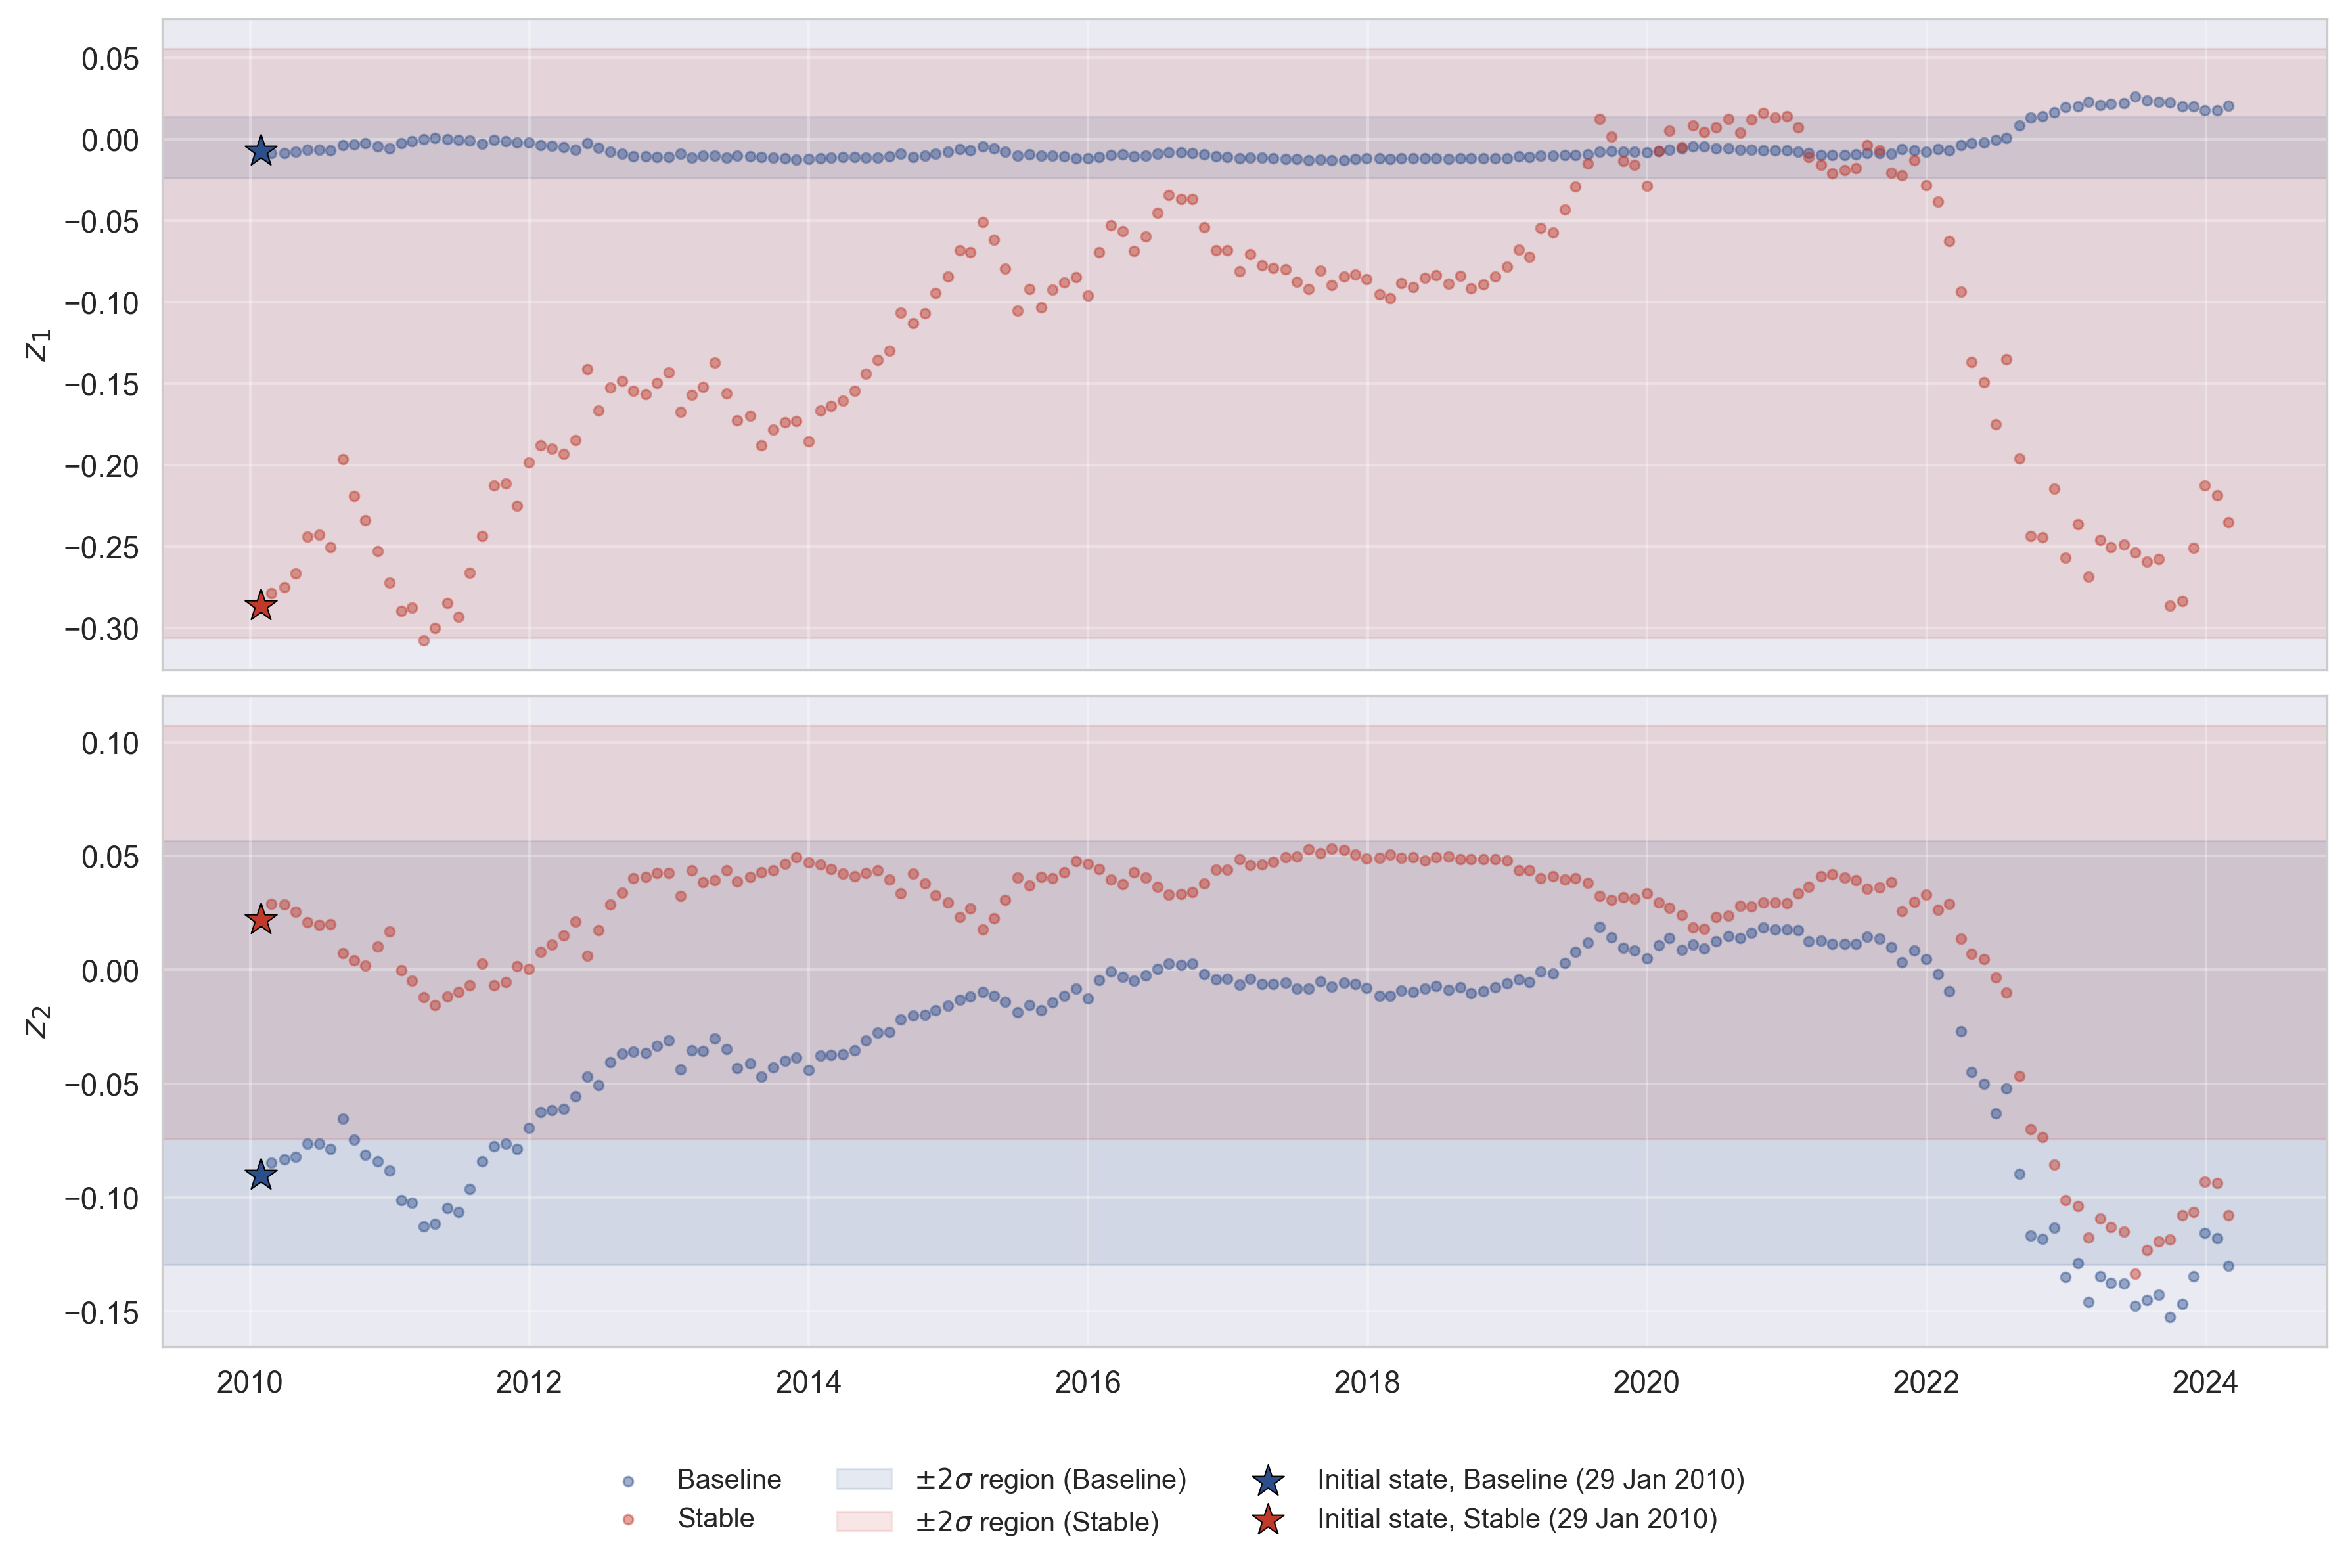
\includegraphics[width=0.95\textwidth]{Figures/Simulation/fig_training_cloud.png}
%\caption{Latent states $z_1$ (top) and $z_2$ (bottom) over the full training period for the baseline and stable models, where each point is the encoding of one observed swap curve. Shaded regions indicate the $\pm 2$ standard deviation range of each model's training data. Stars mark the initial latent state encoded from the EUR swap curve on 29 January 2010, used as the starting point for simulation.}
\caption{Latent states $z_1$ (top) and $z_2$ (bottom) over the full training period for the baseline and stable models, where each point is the encoding of one observed swap curve. Shaded regions indicate the $\pm 2$ standard deviation range of each model's training data. Stars mark the initial latent state encoded from the EUR swap curve on 29 January 2010, used as the starting point for simulation. Despite encoding the same swap curves, the two models map their latent states to different parts of the latent space.}
\label{fig:training_cloud}
\end{figure}

Before examining the simulated paths, Figure \ref{fig:training_cloud} shows the encoded training latent states for both models over the full training period, with the initial state marked. This establishes a reference for the training region, against which the behaviour of simulated paths can be assessed throughout the analysis. 


\begin{description}[
    style=unboxed,
    leftmargin=0pt,
    labelindent=0pt,
    labelsep=0.5em
]


\item[Latent-factor Paths.]

The simulated latent paths, visualized in Figure~\ref{fig:comp_fans}, reveal an immediate contrast between the two models. The baseline paths explode to values of the order \(10^{19}\) by the end of the horizon, far beyond the training region in Figure \ref{fig:training_cloud}, while the stable paths fluctuate throughout but remain bounded. 


\begin{figure}[H]
    \centering
    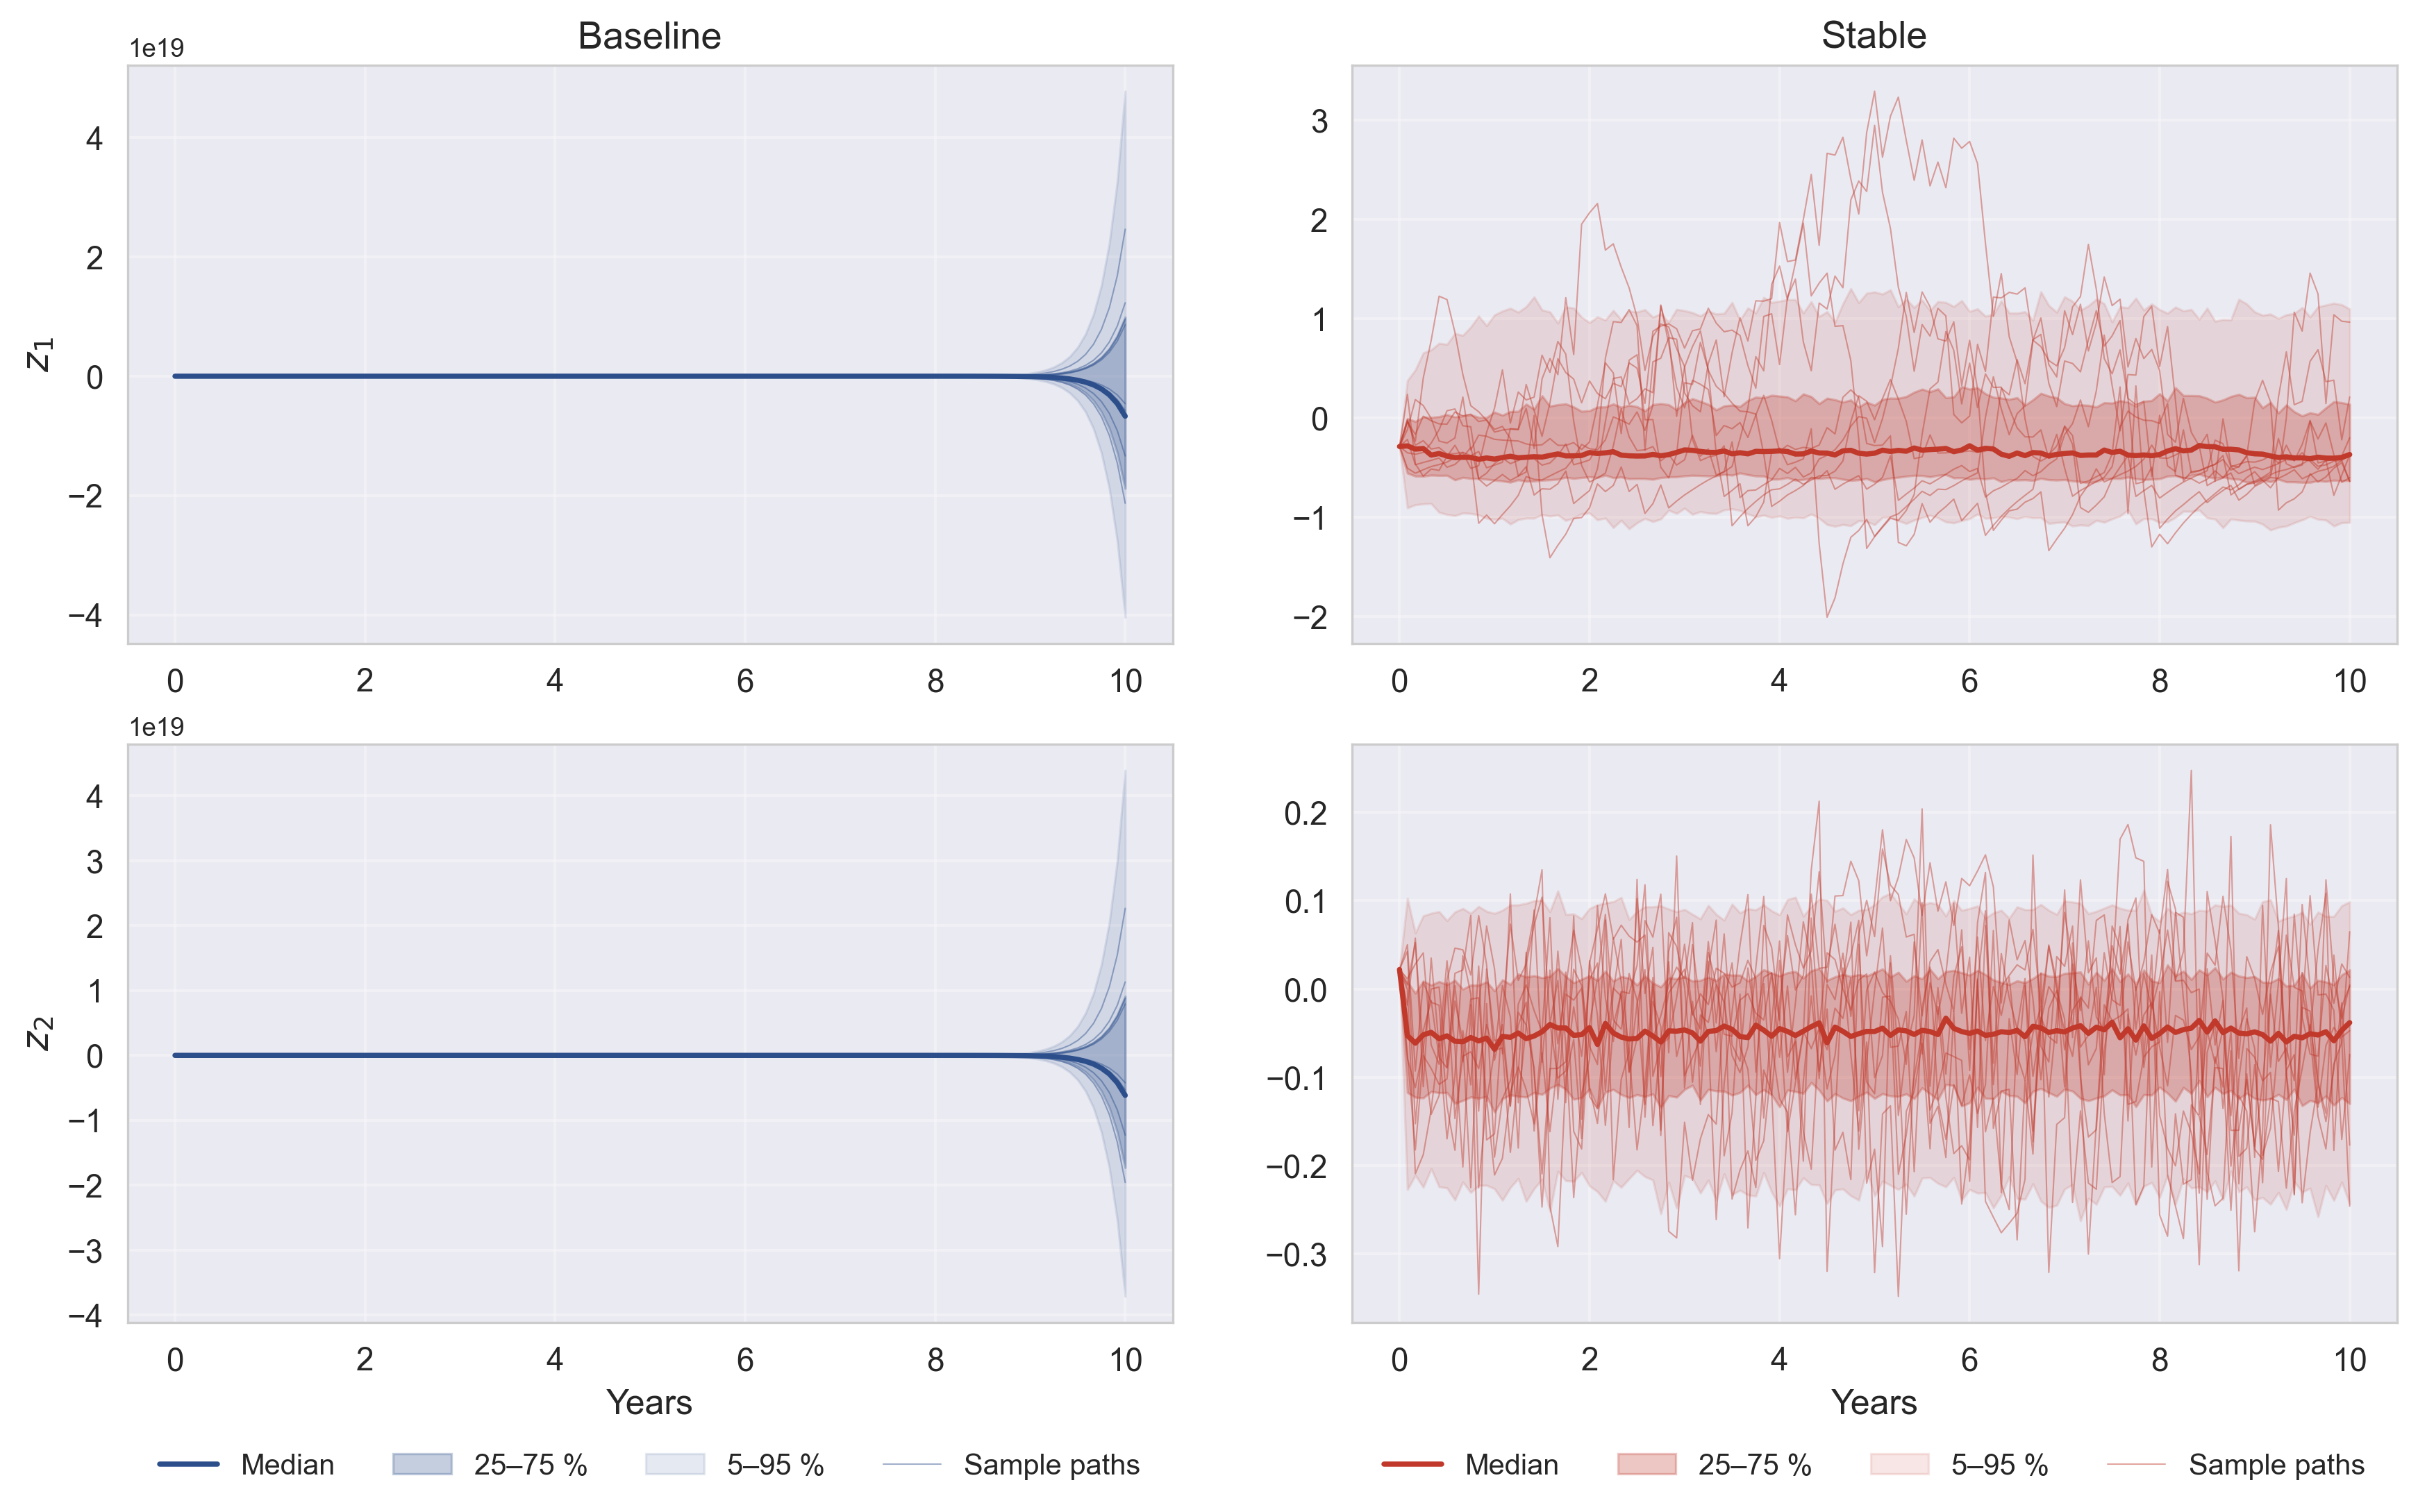
\includegraphics[width=0.95\textwidth]{Figures/Simulation/fig_latent_fans.png}
    \caption{Simulated latent factor paths for $z_1$ (top) and $z_2$ (bottom) over a 10-year horizon, starting from the initial state on 29 January 2010, for the baseline (left) and stable (right) models across $K = 500$ simulations. At each time point, the dark line shows the median across all paths, shaded regions show the 25--75 and 5--95 percentile bands, and 8 individual sample paths are overlaid. The baseline paths explode to values of order $10^{19}$, while the stable model remains bounded throughout.}
    \label{fig:comp_fans}
\end{figure}


The eigenvalues of the learned drift matrix $M$ explain why. By Proposition \ref{prop:meanreversion} in Section \ref{sec:stability_analysis}, mean reversion requires all eigenvalues of $M$ to have negative real parts. The drift matrices of the two trained models have eigenvalues with real parts
\[
\text{Re}(\lambda_1^{\mathrm{base}}) \approx 5.571,
\qquad
\text{Re}(\lambda_2^{\mathrm{base}} )\approx 0.120,
\]
and
\[
\text{Re}(\lambda_1^{\mathrm{stable}}) \approx -1.327,
\qquad
\text{Re}(\lambda_2^{\mathrm{stable}}) \approx -10.846.
\]

Both eigenvalues of the baseline drift matrix have strictly positive real parts, confirming that the baseline model is not mean-reverting, consistent with the $10^{19}$ scale observed in Figure~\ref{fig:comp_fans}. For the stable model, both eigenvalues have strictly negative real parts, so deviations from the fixed
point decay exponentially. The faster reversion of $z_2$, with $|\operatorname{Re}(\lambda_2^{\mathrm{stable}})| \approx 10.846$ versus $|\operatorname{Re}(\lambda_1^{\mathrm{stable}})| \approx 1.327$, is reflected in its tighter range in Figure~\ref{fig:comp_fans}.


For each latent factor \(\ell=1,2\), Figure~\ref{fig:log_growth} gives a complementary view by plotting 
\[
\log_{10}\left(
\frac{1}{K}\sum_{k=1}^{K}|z_\ell^{(k)}(t)|
\right),
\]
where \(z_\ell^{(k)}(t)\) denotes latent factor \(\ell\) on simulated path \(k\). Exponential growth appears approximately linear on this scale. The baseline paths follow this pattern closely, while the stable curves level off.

\begin{figure}[H]
    \centering
    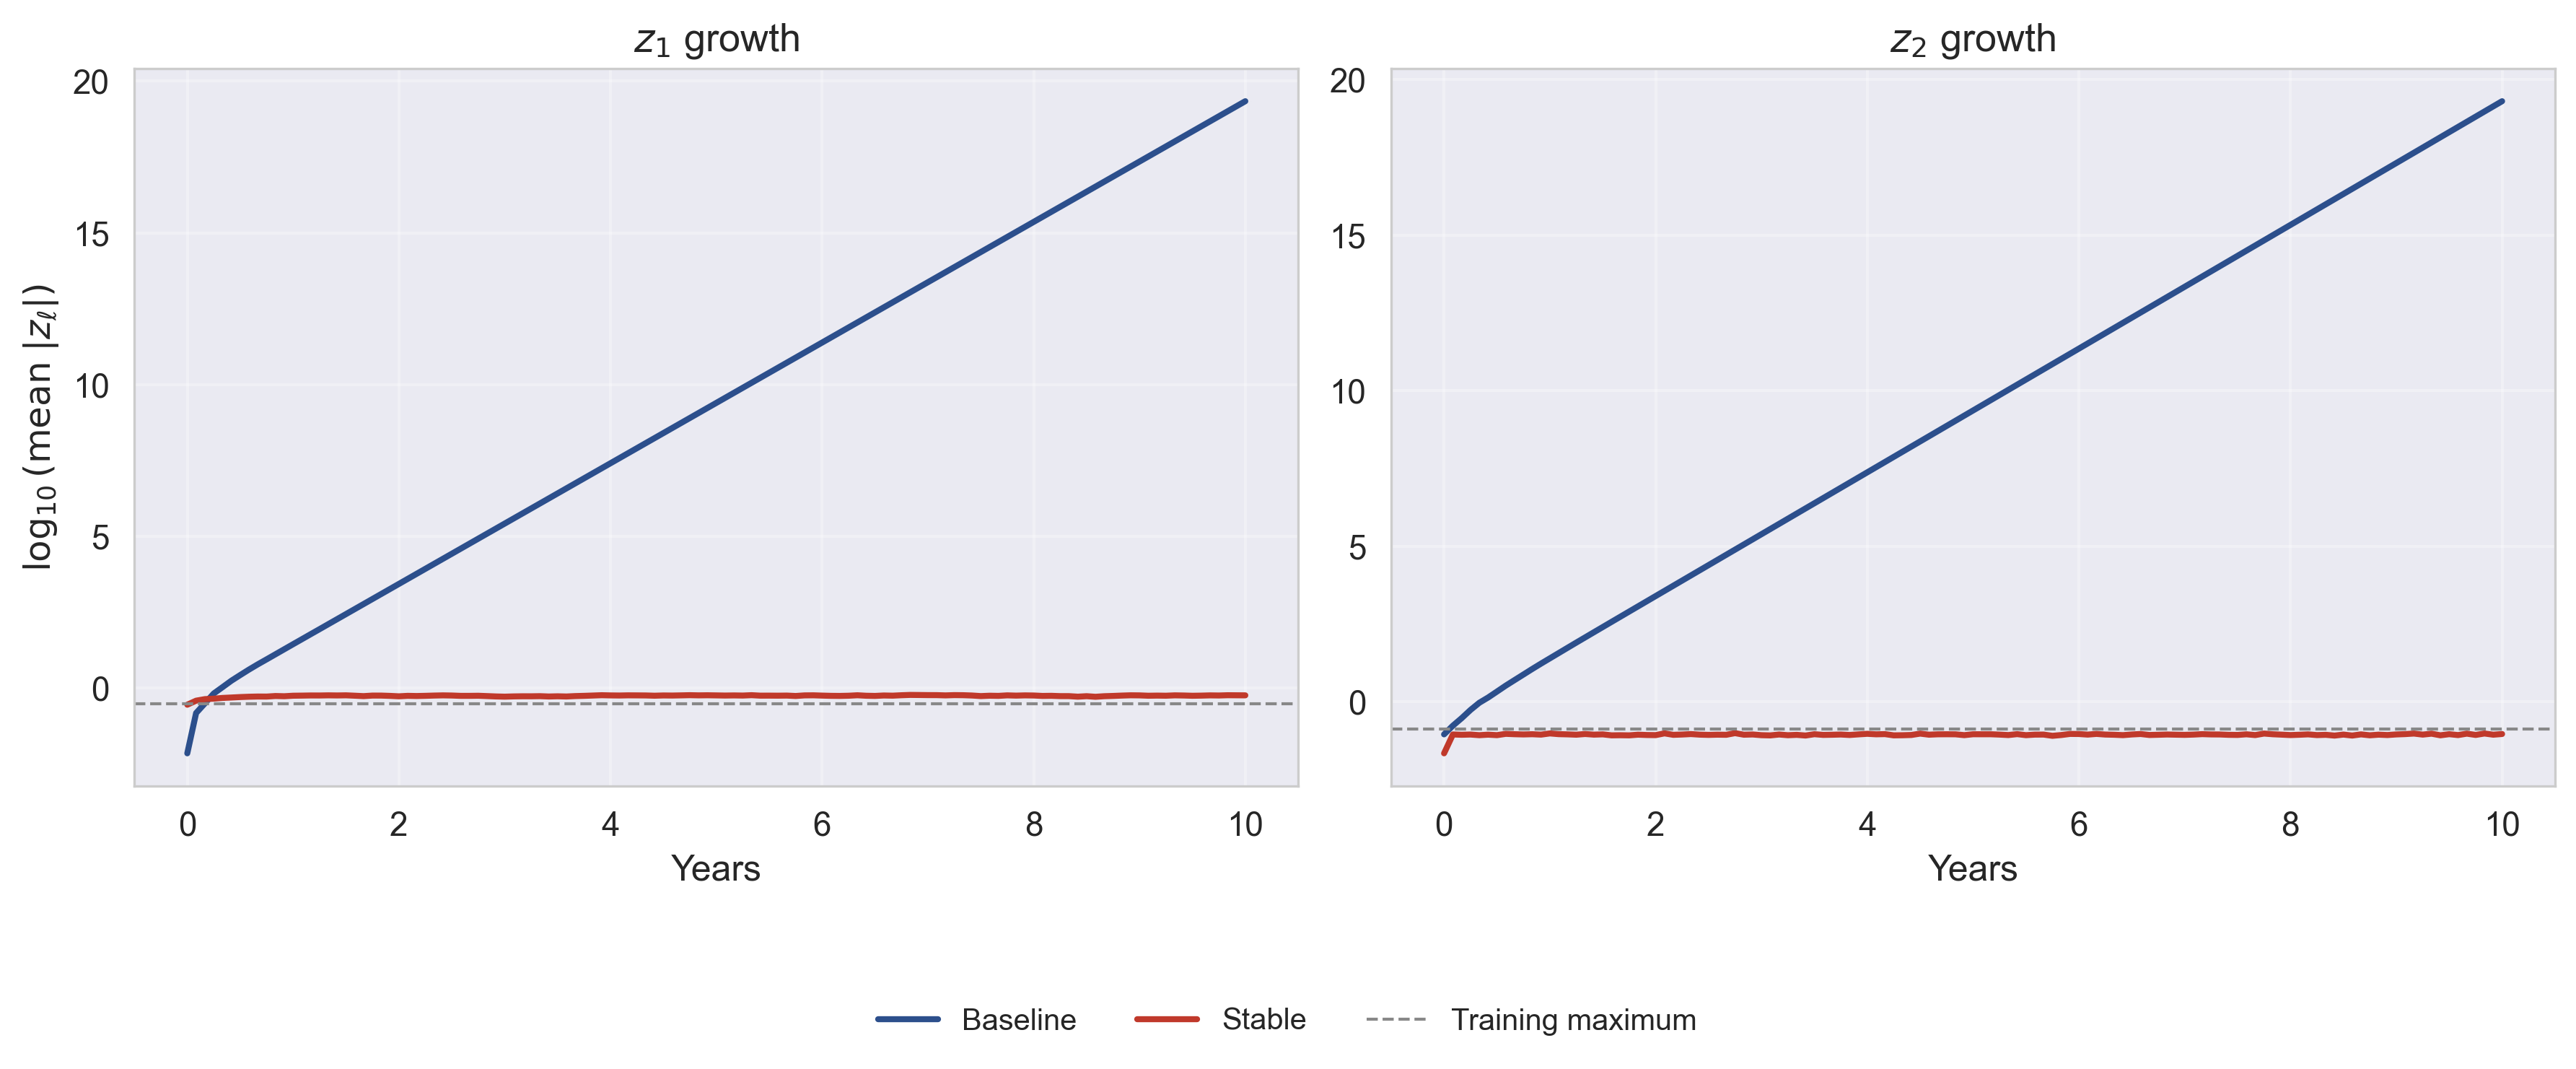
\includegraphics[width=0.9\textwidth]{Figures/Simulation/fig_log_growth.png}
    \caption{$\log_{10}(\operatorname{mean}|z_\ell(t)|)$ over a 10 year simulation horizon for $z_1$ (left) and $z_2$ (right), for the baseline and stable models. The baseline grows approximately linearly on the log scale, indicating exponential growth in the latent factors. The stable model remains close to the training data range throughout, with the dashed line marking the maximum of $|z_\ell|$ observed in the training data.}
    \label{fig:log_growth}
\end{figure}

To summarise, the baseline drift violates the mean reversion condition of Proposition \ref{prop:meanreversion}, producing paths that grow exponentially. The stable model prevents this.



\item[Short-rate behaviour.] We next examine how the latent path behaviour affects the simulated short rate in Figure \ref{fig:comp_short_rate_fan}.

\begin{figure}[H]
    \centering
    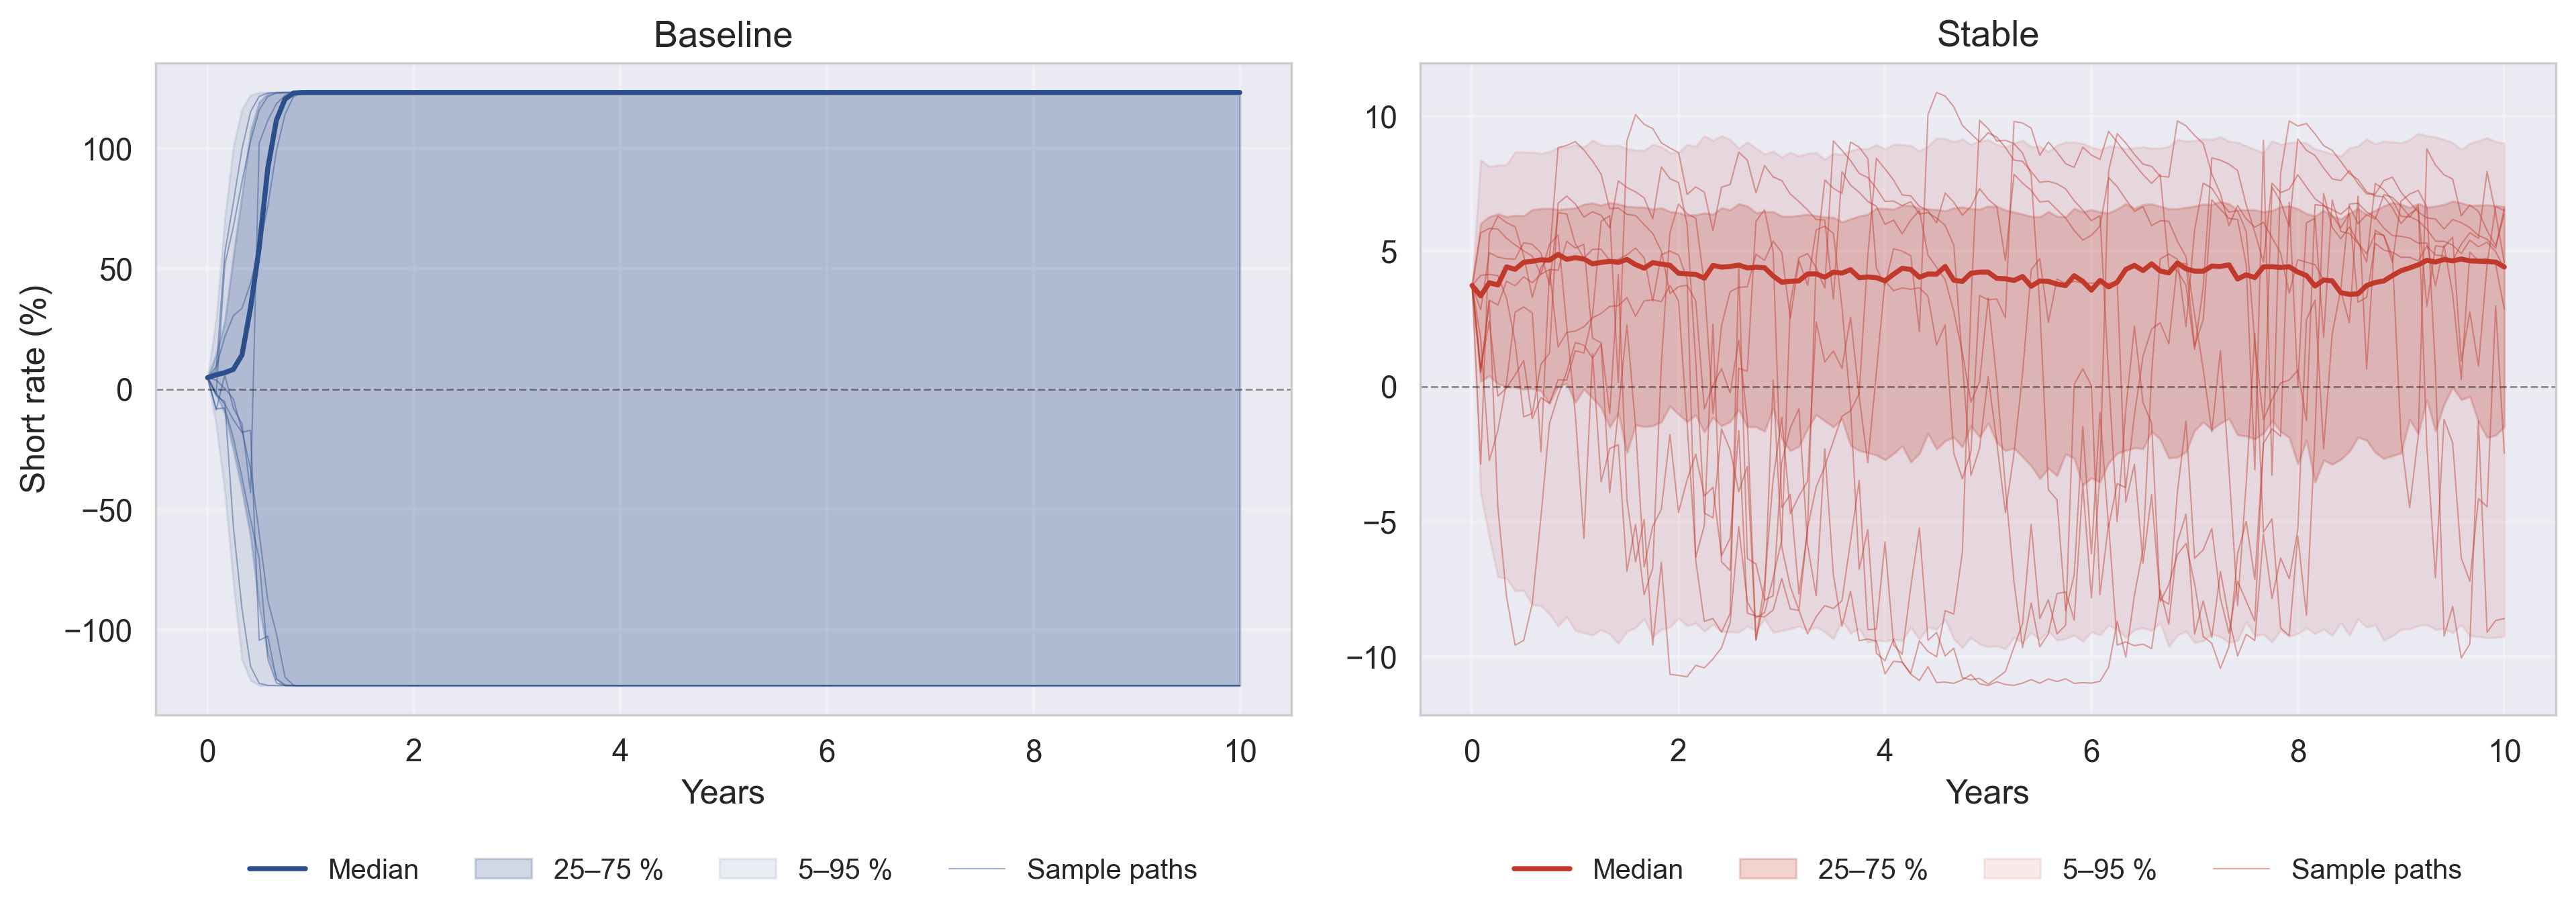
\includegraphics[width=0.9\textwidth]{Figures/Simulation/fig_short_rate_fan.png}
    \caption{Simulated short rate $\tilde{r}(z_t)$ (\%) over a 10-year horizon, starting from the initial state on 29 January 2010, for the baseline (left) and stable (right) models across $K = 500$ simulations. At each time point, the dark line shows the median across all paths, shaded regions show the 25--75 and 5--95 percentile bands, and 8 individual sample paths are overlaid. The baseline short rate explodes to values exceeding $\pm$100\% within the first two years, while the stable model remains bounded throughout.}
    \label{fig:comp_short_rate_fan}
\end{figure}

As the baseline latent paths move to extreme regions of latent space, the activation function of the short rate network saturates, pinning the short rate near an implied ceiling or floor. Within approximately one year of simulating forward, the baseline median is flat near its upper limit, with percentile bands spanning approximately $[-125\%, 125\%]$. The stable short rate, by contrast, remains within the range of approximately $[-11\%, +11\%]$ throughout the horizon.

\textcolor{red}{The stable short rate, by contrast, remains within the range of approximately $[-11\%, +11\%]$ throughout the horizon,  considerably wider than historically observed short rates, reflecting that the model learns a conservative bound rather than real market levels.}


\item[Terminal distributions.] 

Beyond how paths evolve over time, Figure~\ref{fig:comp_terminal} examine the terminal distribution of both the latent states and the short rates at $T=10$ years.

\begin{figure}[H]
    \centering
    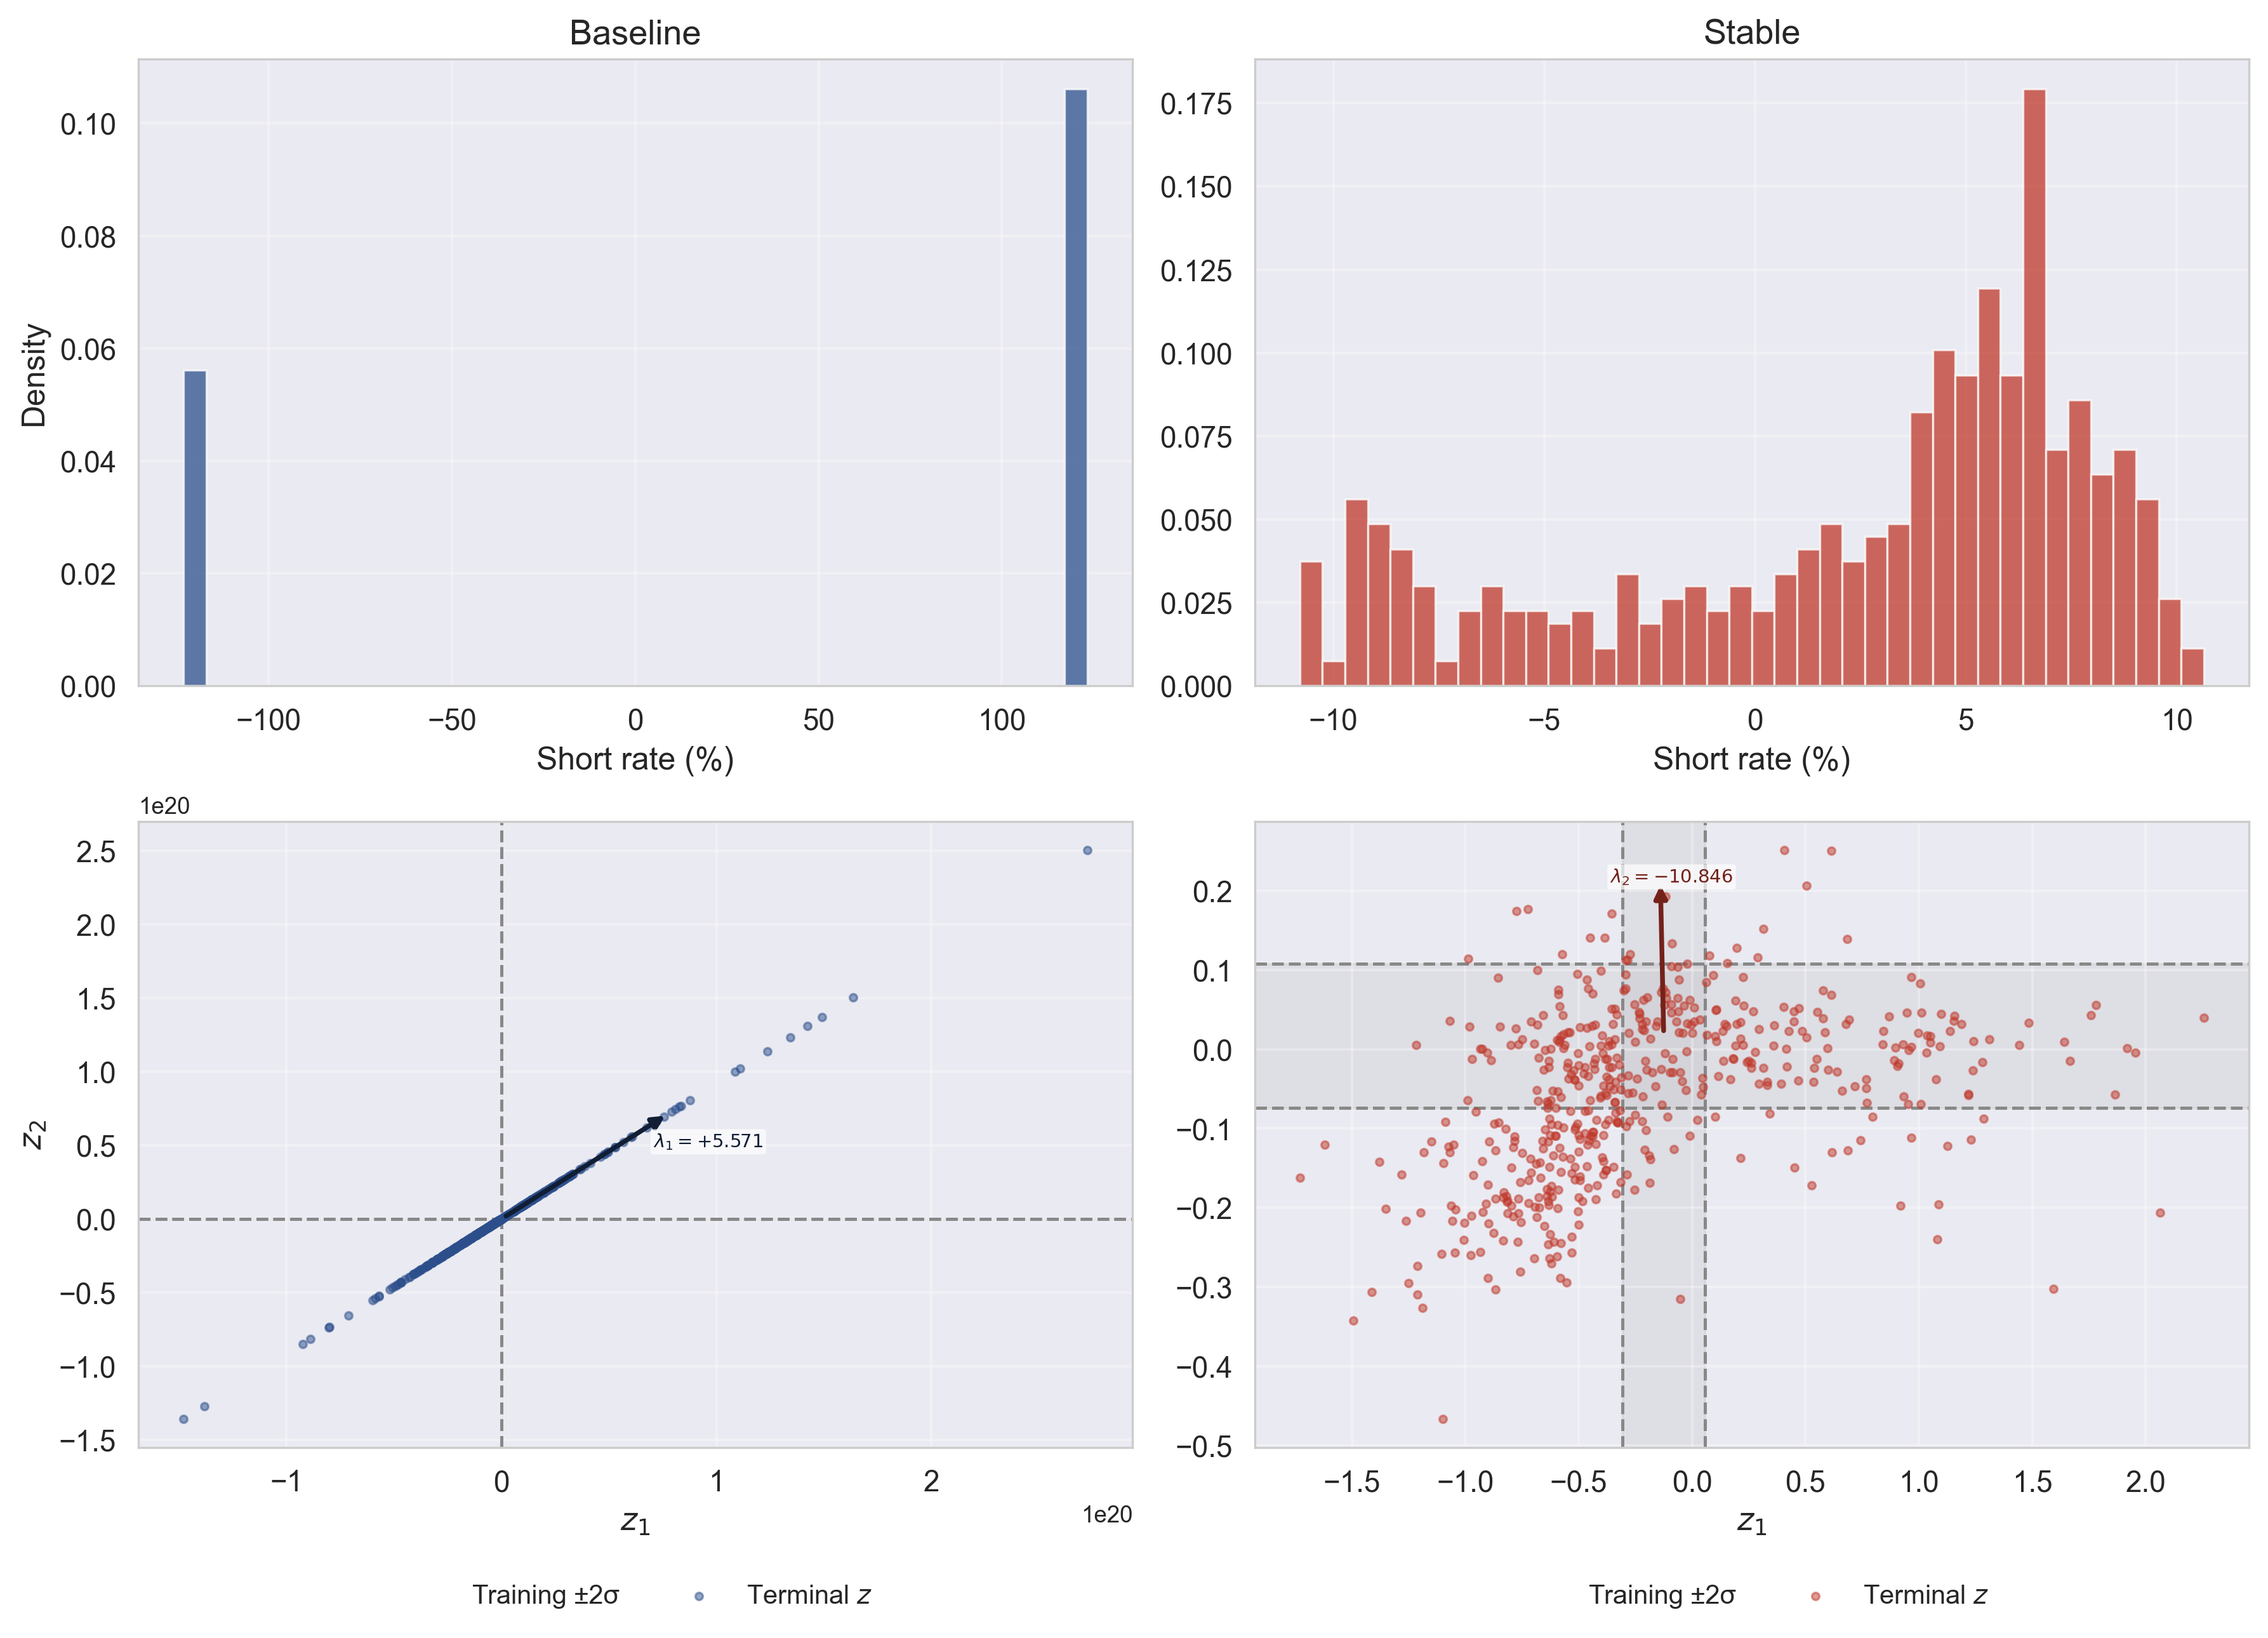
\includegraphics[width=\textwidth]{Figures/Simulation/fig_terminal_dist.png}
    \caption{Terminal distributions at $T = 10$ years for the baseline (left) and stable (right) models. Top row: histograms of the terminal short rate $\tilde{r}(z(T))$. Bottom row: scatter of terminal latent states $(z_1, z_2)$, with the shaded box marking the $\pm 2$ standard deviation range of each model's training data. The arrow indicates the dominant eigenvector of the drift matrix $M$, annotated with the real part of the corresponding eigenvalue; a positive real part indicates a diverging process while a negative real part indicates mean reversion. The baseline terminal states lie far outside the training region at values of order $10^{20}$, while most stable model terminal states remain within it.}
    \label{fig:comp_terminal}
\end{figure}


For the baseline, the terminal latent state collapse onto a straight line. The arrow indicates the dominant eigenvector of $M$, annotated with $\text{Re}(\lambda_1^{\text{base}})=+5.571$, the eigenvalue with the larger absolute real part. Because the real part of the eigenvalue is positive, any component along it grows without bound, and after ten years all paths are dominated by that single direction of growth. The short-rate histogram reflects this degeneracy, with all mass concentrated at extreme values near \(\pm125\%\).

The stable terminal latent states form a diffuse cloud rather than collapsing onto a single direction. Since both real parts are strictly negative, no single direction of growth dominates, and the terminal short-rate distribution spans a range of approximately $[-11\%, 11\%]$, which is considerably more plausible than the baseline range of $\pm 125\%$.


\item[Volatility bounds.] The volatility function scales the Brownian shock, and large values can cause simulated paths to diverge over long horizons. To assess how the learned volatility function behaves away from the training region, each model is evaluated on two sets of latent states. The first is the encoded training cloud, visualised over time in Figure~\ref{fig:training_cloud}. The second is an expanded set, constructed by sampling around the training cloud mean with three times the empirical latent standard deviation.

\begin{table}[H]
\centering
\small
% Auto-generated by stable_vs_baseline_results.py — do not edit by hand.
\begin{tabular}{@{}llcc@{}}
\toprule
\textbf{Factor} & \textbf{Evaluation set} & \textbf{Baseline} & \textbf{Stable} \\
\midrule
\(\sigma_1(z)\) & Encoded training cloud & \([0.5101,\,1.0873]\) & \([0.0288,\,1.7269]\) \\
\(\sigma_1(z)\) & Expanded diagnostic set & \([0.1563,\,4.4862]\) & \([0.0003,\,1.9949]\) \\
\midrule
\(\sigma_2(z)\) & Encoded training cloud & \([0.4847,\,1.0975]\) & \([0.2598,\,0.3483]\) \\
\(\sigma_2(z)\) & Expanded diagnostic set & \([0.1384,\,4.9840]\) & \([0.1596,\,0.4955]\) \\
\bottomrule
\end{tabular}


\caption{Min--max ranges of the volatility functions $\sigma_i(z)$ evaluated at the training latent states and at an expanded diagnostic set drawn from $\mathcal{N}(\mu_{\mathrm{train}},\, (3\sigma_{\mathrm{train}})^2)$. The expanded set probes behaviour outside the training region to assess whether the volatility functions remain bounded under extrapolation.}
\label{tab:sigma_ranges}
\end{table}

Table~\ref{tab:sigma_ranges} reports the volatility ranges over both evaluation sets. For the stable model, the ranges do widen on the expanded diagnostic set, but only marginally so, remaining within the prescribed bounds $\sigma_{\min}$ and $\sigma_{\max}$. For the baseline model, the picture is very different, with both $\sigma_1$ and $\sigma_2$ approaching values near $5$ on the expanded set against roughly $1.1$ on the training cloud. 

It is worth noting that the stable $\sigma_1$ reaches $1.9949$ on the expanded set, approaching the chosen hyperparameter $\sigma_{\max} = 2$, which suggests that a more careful calibration of the bounds would be warranted in practice. We do not investigate this further here.


\item[Decoded swap-rate curves.] That latent instability matters in practice is even more clear when the simulated states are decoded back into swap rate curves. Figure \ref{fig:yield_curves} shows decoded curves at $t=1,5$ and $10$ years for both models.

\begin{figure}[H]
    \centering
    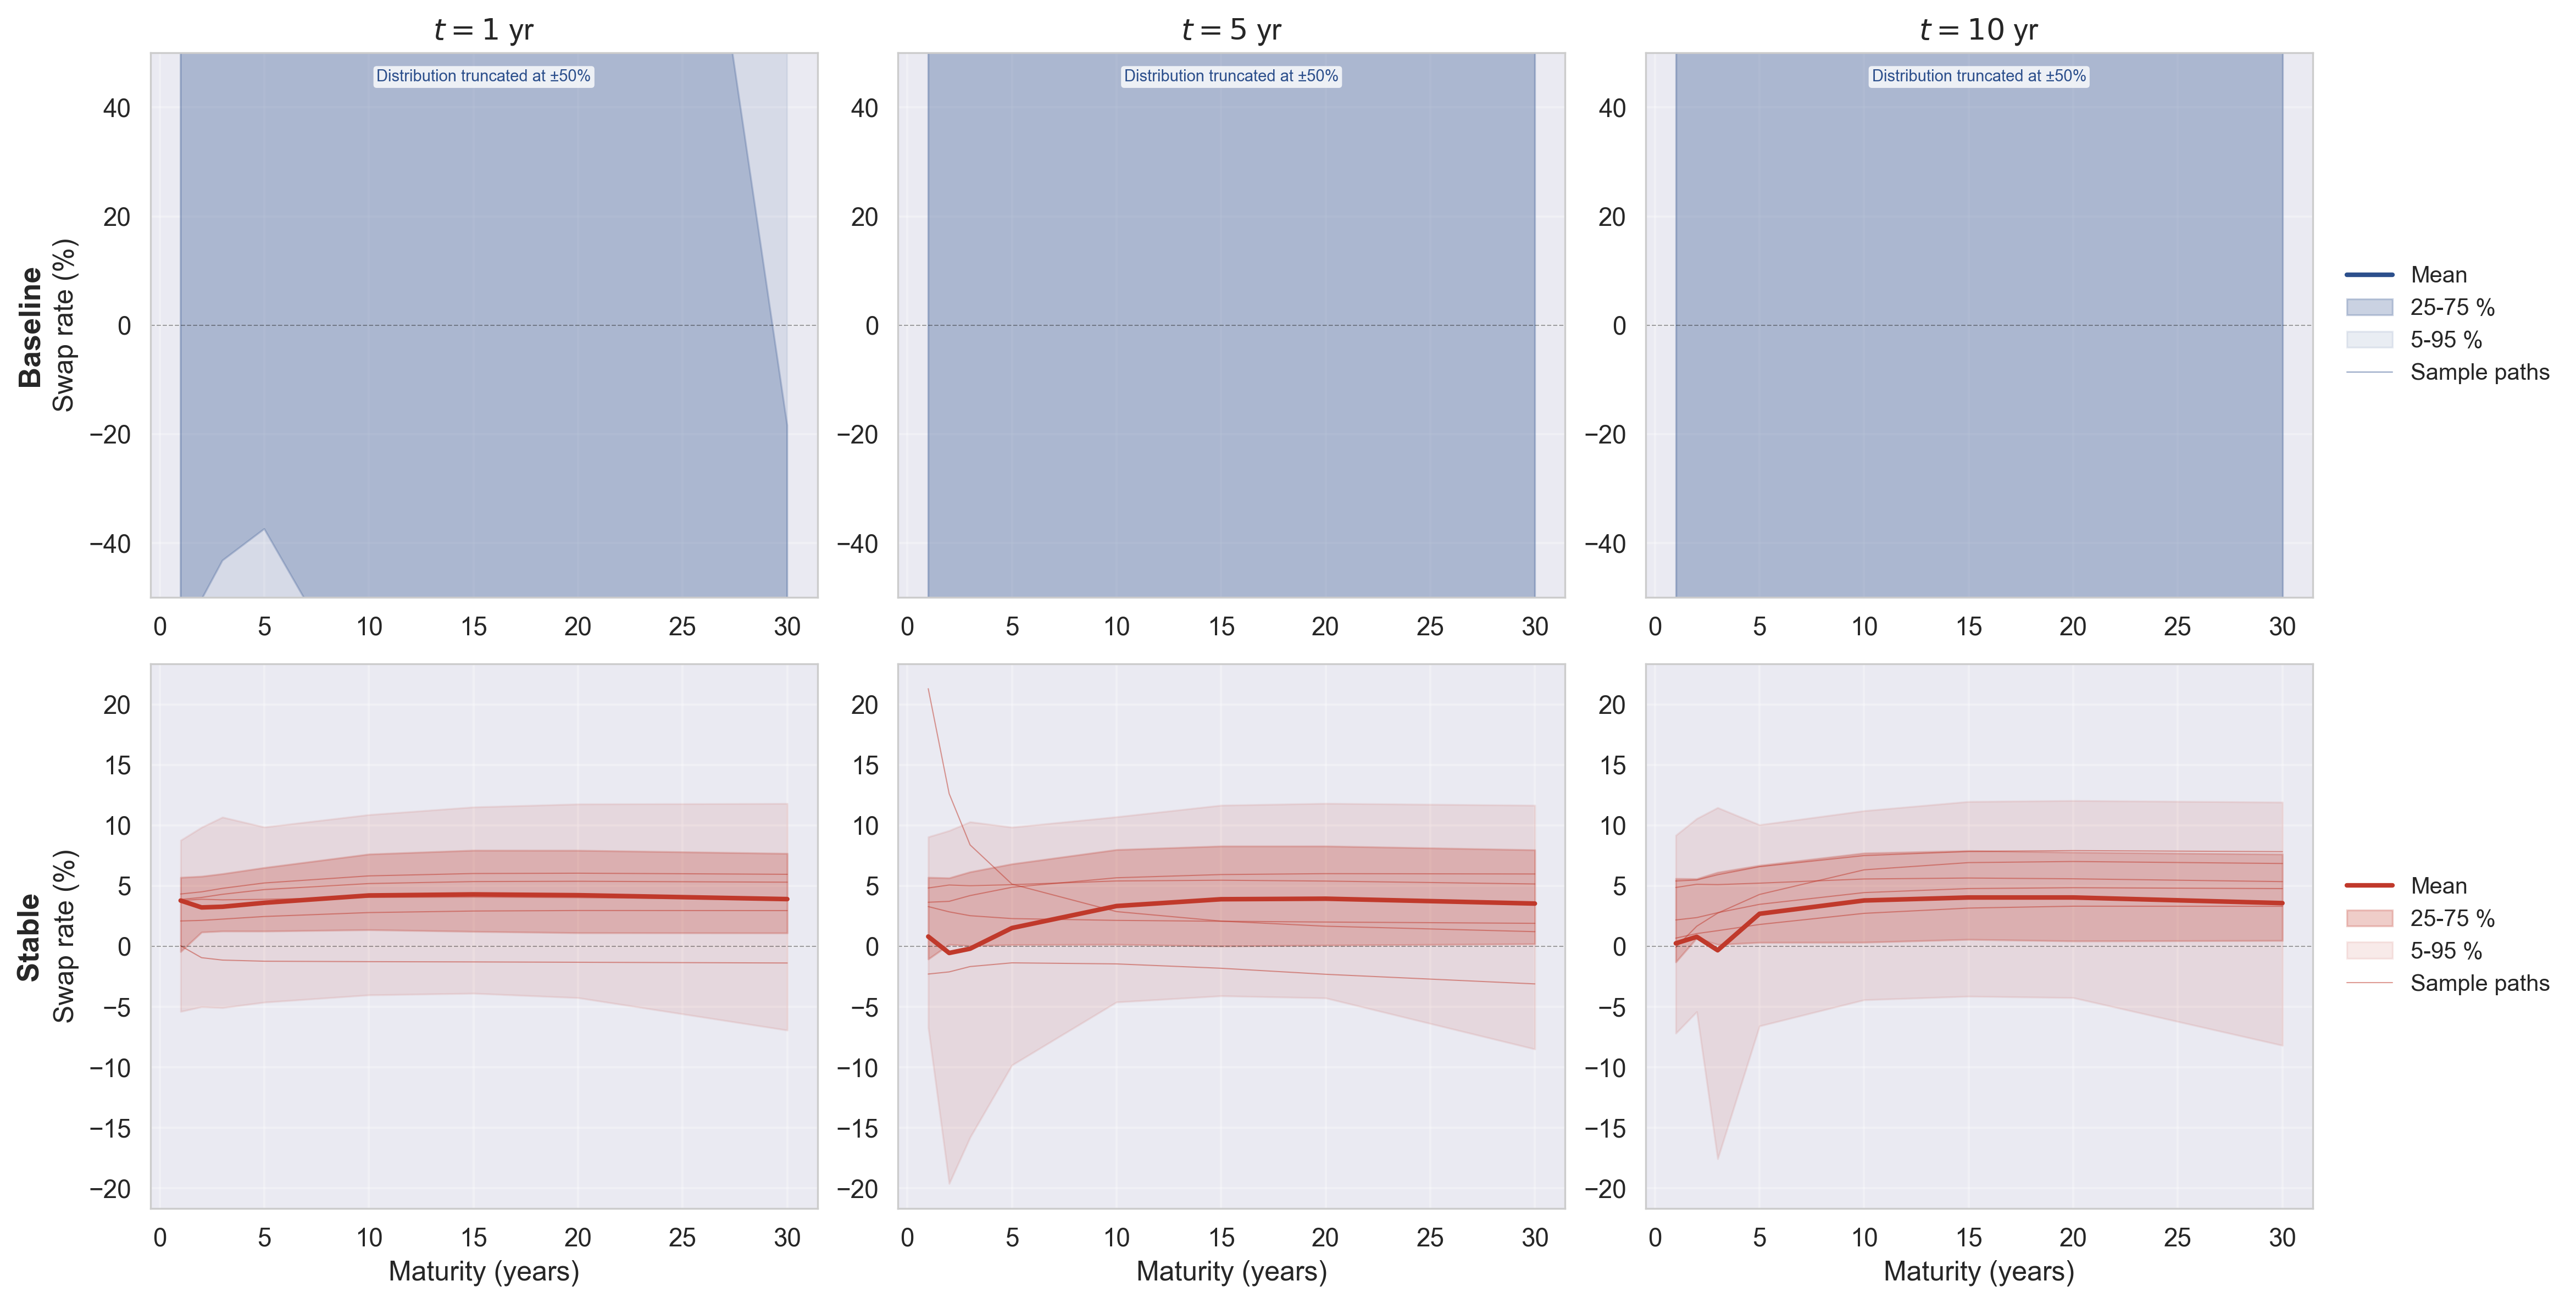
\includegraphics[width=\textwidth]{Figures/Simulation/fig_yield_curves.png}
    \caption{Swap-rate curves decoded from simulated latent states, shown at $t = 1$, $5$, and $10$ years for the baseline (top) and stable (bottom) models. At each time point, the latent state $z_t$ from each simulated path is passed through the decoder to produce a swap-rate curve; each panel summarises the resulting distribution across $K = 500$ paths as the mean, 25th--75th and 5th--95th percentile bands, with 5 individual paths overlaid. The baseline panels are clipped at $\pm 50$ percentage points, as the distribution diverges far beyond this range. The stable model panels share a common y-axis scale, remaining within a range consistent with historical swap rates throughout the full $T = 10$ year simulation.}
    \label{fig:yield_curves}
\end{figure}
The baseline distribution exceeds the display range of $\pm 50$ percentage points already at $t = 1$. So the shape of the simulated curves cannt be assessed directly. Nevertheless, swap rates of this magnitued are far outisde any historically observed range, confirming that the decoder is operating on latent states never encountered during training.The stable model, by contrast, produces curves that remain within a range consistent with historical swap rates throughout the full $T = 10$ year simulation.
\end{description}


The experiment demonstrates that the stability constraints on the drift, diffusion, and short-rate output jointly ensure that simulated paths and decoded curves remain on an interpretable scale throughout the ten-year horizon.



%========================================================
\section{Reconstruction Accuracy of the Stable Model}
\label{sec:sim_reconstruction_accuracy}
%========================================================
Imposing stability restrictions improves simulation behaviour. This section examines whether doing so has any impact on reconstruction accuracy. The baseline and stable models are compared across latent dimensions $\ell\in\{2,3,4\}$ using a multi-currency rolling out-of-sample framework following the protocol from Chapter~\ref{chap:evaluation}.

\begin{table}[H]
\centering
{\small
\begin{tabular}{@{}llrrr@{}}
\toprule
\textbf{\(\ell\)} & \textbf{Model} & \textbf{Avg. IS} & \textbf{Avg. OOS} & \textbf{Max OOS }\\
\midrule
    2 & Baseline & 10.5 & 19.0 & 77.0 \\
    2 & Stable & 138.7 & 127.6 & 1811.7 \\
    \midrule
    3 & Baseline & 11.6 & 66.5 & 632.6 \\
    3 & Stable & 10.5 & 21.6 & 145.7 \\
    \midrule
    4 & Baseline & 9.3 & 100.5 & 691.8 \\
    4 & Stable & 8.1 & 12.1 & 24.2 \\
    \bottomrule

%\bottomrule
\end{tabular}
}
\caption{In-sample and out-of-sample RMSE (bps) for the baseline and stable models at latent dimensions $\ell \in \{2, 3, 4\}$, evaluated across 18 rolling windows with 5-year training and 6-month test periods. Avg.\ IS is the average RMSE across the 18 training windows. Avg.\ OOS and Max OOS are the average and maximum RMSE across the 18 test windows. All models are trained for $3{,}500$ epochs. While the stable model fails to reconstruct accurately at $\ell = 2$, it outperforms the baseline out of sample from $\ell = 3$ onward, with $\ell = 4$ achieving the best overall out-of-sample performance.}
\label{tab:oos_summary_sim}
\end{table}

Whether the stability restrictions improve reconstruction accuracy depends strongly on the latent dimension, as shown in Table \ref{tab:oos_summary_sim}. At $\ell=2$, the stable model struggles severely, with an average IS RMSE of $138.7$ bps against $10.5$ bps for the baseline, suggesting the restrictions are too constraining relative to the available latent degrees of freedom. From $\ell=3$ onward, the stable model improves substantially. 

As established in Chapter~\ref{chap:evaluation}, the baseline overfits for latent dimensions larger than two, and this is reflected here in its out-of-sample RMSE increasing from $19.0$ bps at $\ell=2$ to $100.5$ bps at $\ell=4$. The stable model moves in the opposite direction, and at $\ell=4$ achieves the lowest average and maximum out-of-sample RMSE across all configurations. At $12.1$ bps out-of-sample, it improves upon the best baseline configuration, $\ell=2$ at $19.0$ bps. The stability restrictions therefore do not come at the cost of worsened reconstruction accuracy. With sufficient latent dimensions, they improve it.

The aggregate results in Table \ref{tab:oos_summary_sim}, however, mask how reconstruction accuracy varies across the sample. Figure~\ref{fig:rolling_oos_rmse} plots the rolling out-of-sample RMSE over time for all three latent dimensions, allowing a direct comparison of how each model behaves across different rate environments present in the data.

\begin{figure}[H]
    \centering
    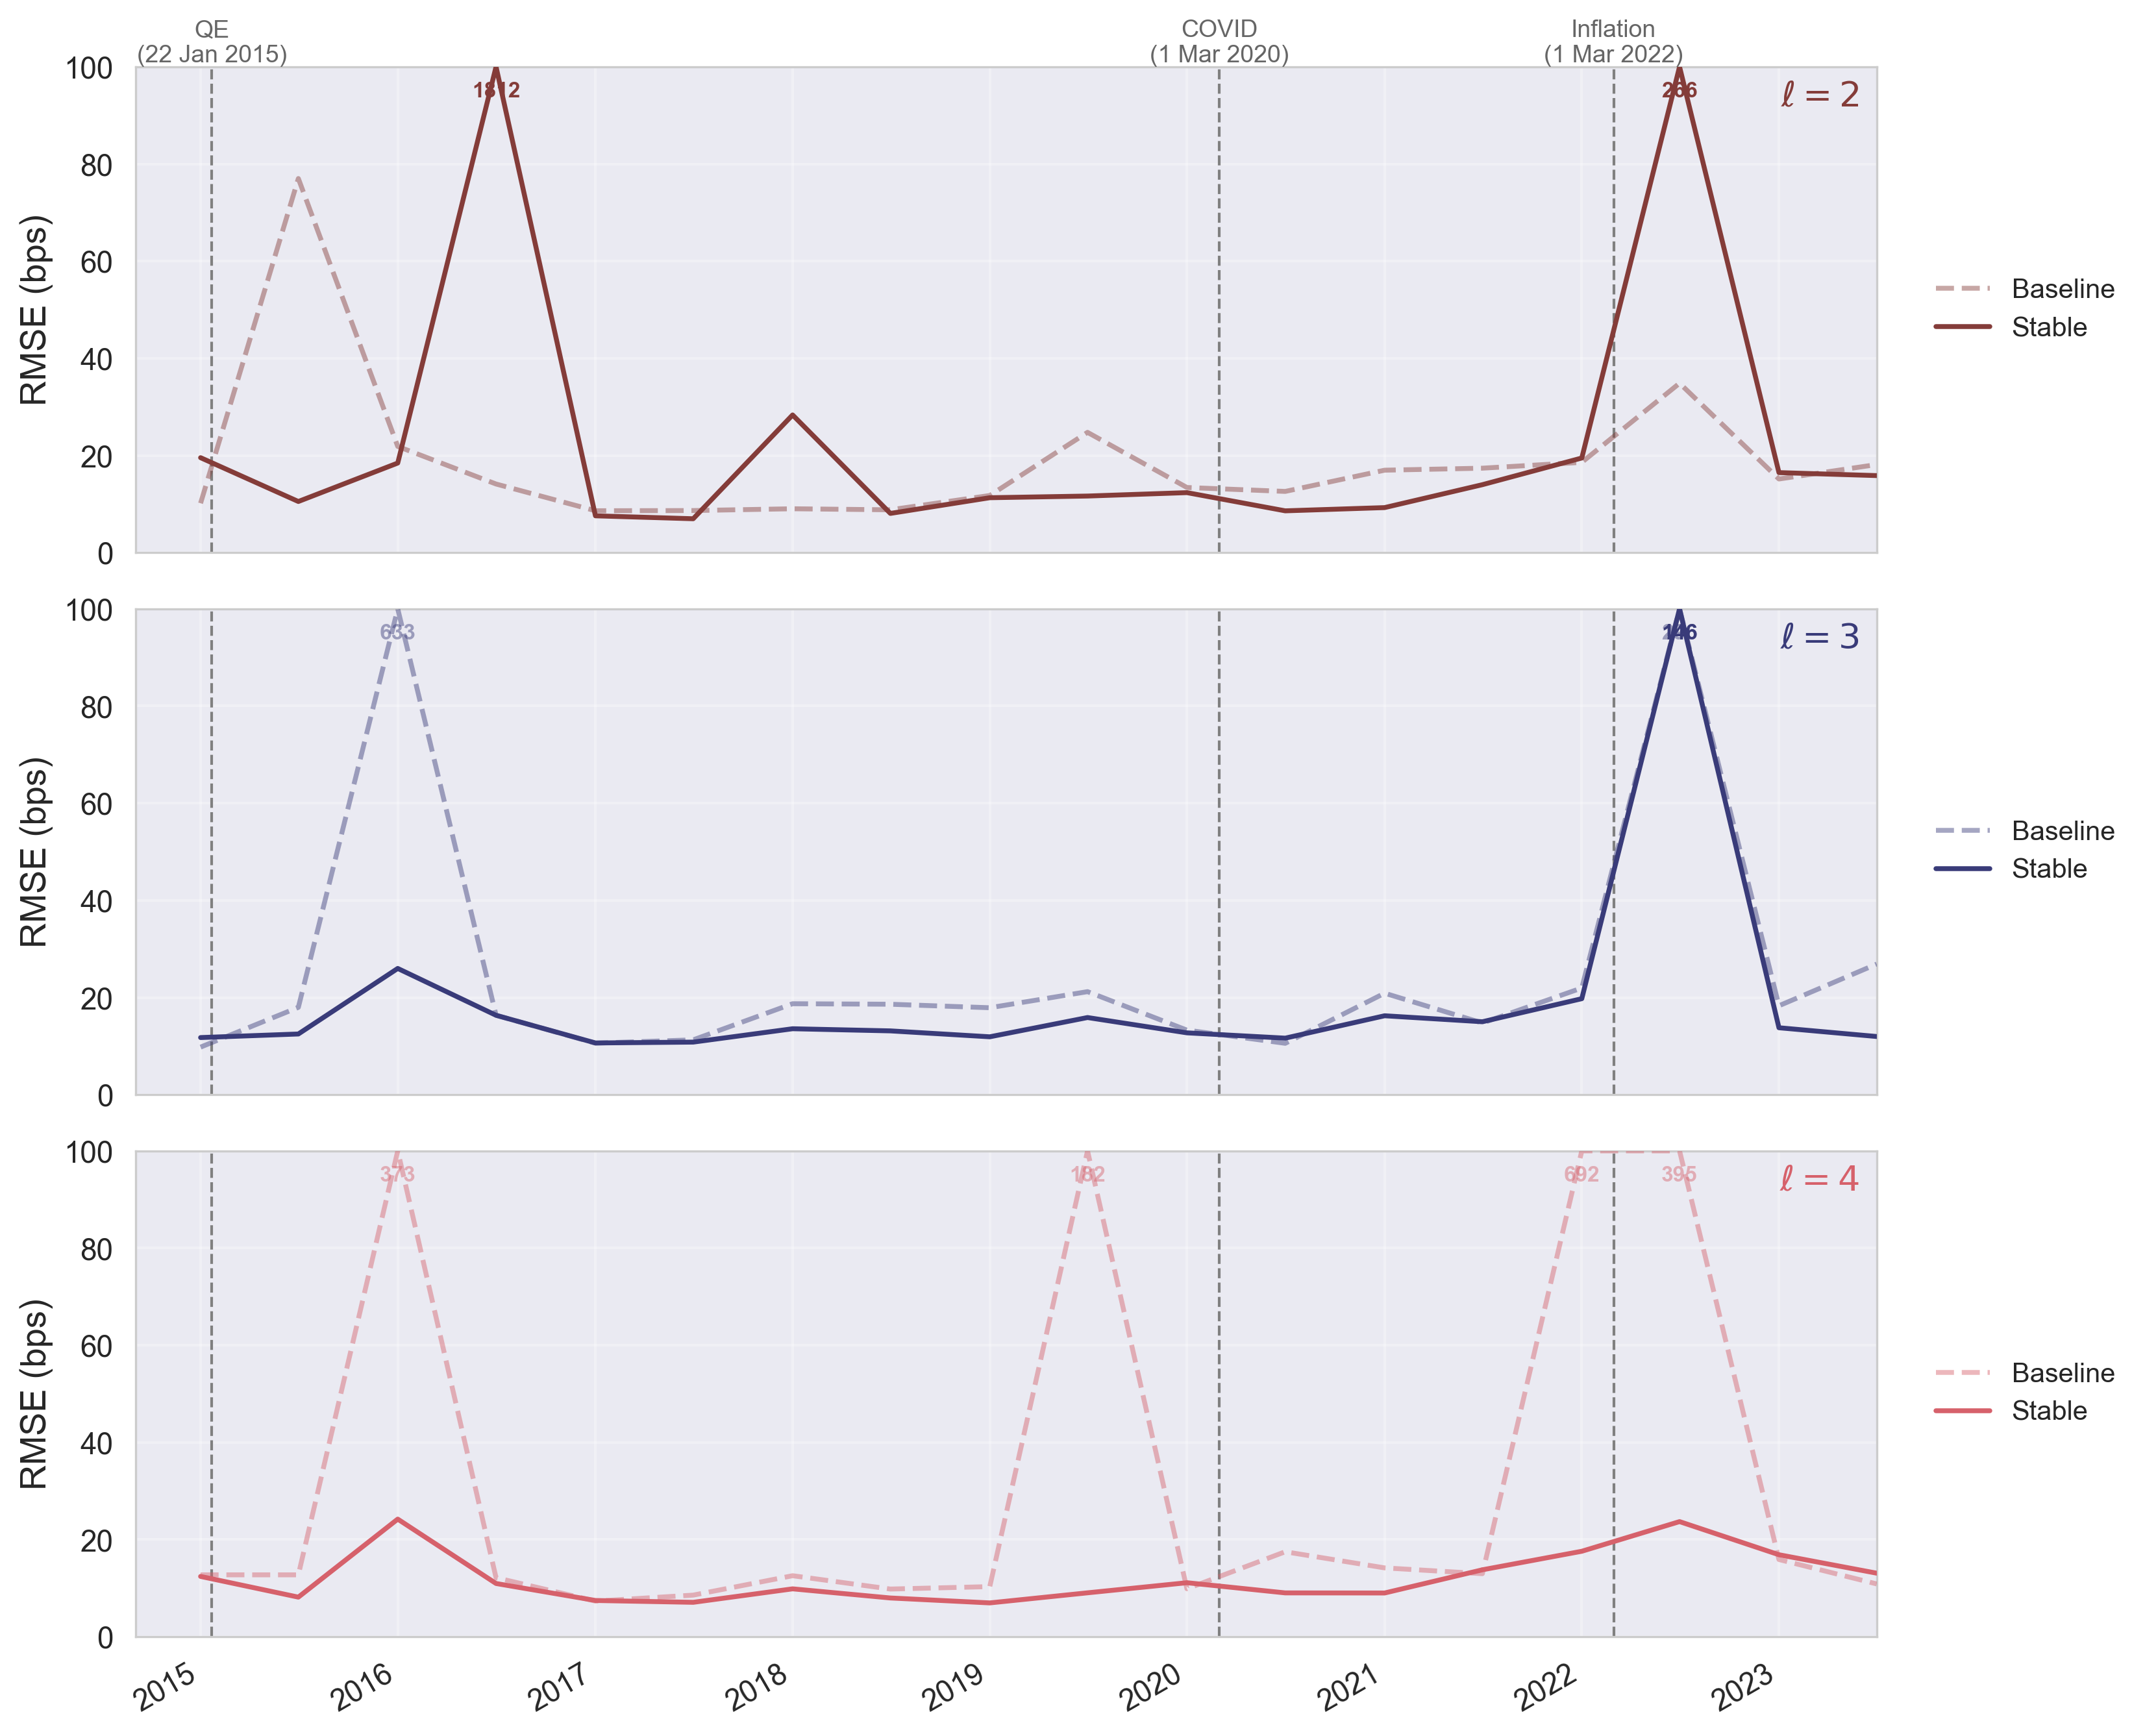
\includegraphics[width=\textwidth]{Figures/Simulation/fig_rolling_rmse.png}
    \caption{Rolling out-of-sample RMSE (bps), averaged across currencies, for the baseline (dashed) and stable (solid) models at latent dimensions $\ell \in \{2, 3, 4\}$. Each point reports the average RMSE across all curve observations in a six-month test window. The y-axis is clipped at 100 bps. Annotated values show the true RMSE where clipping occurs. Grey vertical lines mark the onset of macroeconomic regimes. At \(\ell=3\) and \(\ell=4\), the stable model consistently outperforms the baseline throughout the sample, with the largest improvements during the spike periods around 2016 and 2022.}
    \label{fig:rolling_oos_rmse}
\end{figure}


As established in Chapter~\ref{chap:evaluation}, the baseline struggles most severely when the share of curve types in the test set substantially exceeds that in the training window, most notably around the quantitative easing regime in 2015 and the inflation regime beginning in 2022. At $\ell=4$, the stable model maintains a consistently low error on average throughout the sample, with only modest increases around these episodes, indicating that it handles the underrepresented curves better.

A more detailed breakdown by curve type is provided in Chapter~\ref{chap:model_comparison}. For now, the rolling out-of-sample comparison confirms that with $\ell=4$, the stable model 
handles shifts in the rate environment considerably better than the baseline.












